% ****** Start of file aipsamp.tex ******
%
%   This file is part of the AIP files in the AIP distribution for REVTeX 4.
%   Version 4.1 of REVTeX, October 2009
%
%   Copyright (c) 2009 American Institute of Physics.

% Use this file as a source of example code for your aip document.
% Use the file aiptemplate.tex as a template for your document.
\documentclass[%
 aip,
 jmp,%
 amsmath,amssymb,
%preprint,%
 reprint,%
 floatfix,
%author-year,%
%author-numerical,%
]{revtex4-1}
\usepackage{graphicx}% Include figure files
\usepackage{grffile}
\usepackage{dcolumn}% Align table columns on decimal point
\usepackage{bm}% bold math
%\usepackage[mathlines]{lineno}% Enable numbering of text and display math
%\linenumbers\relax % Commence numbering lines
\maxdeadcycles=1000
\usepackage{multirow}
\usepackage{color} % for the notes
\usepackage{etex}
\usepackage{float}
\usepackage{pgffor}
\usepackage{morefloats}
\reserveinserts{358}
%\extrafloats{1000}
\usepackage{hyperref}
\usepackage[usenames,dvipsnames]{xcolor}
\usepackage{amsmath}
\hypersetup{
        colorlinks,
        linkcolor={red!50!black},
        citecolor={blue!50!black},
        urlcolor={blue!80!black}
}
\usepackage{longtable}
\usepackage{float}
\usepackage{supertabular}

\usepackage{booktabs}
\usepackage{array}
 
%\usepackage{placeins}
\usepackage{xr}
\externaldocument{paper}
\usepackage[section] {placeins}

\newcommand{\minput}[1]{%
\IfFileExists{#1}{\input{#1}}{}
}

\newcommand{\finput}[1]{%
\IfFileExists{#1}{
\begin{figure}[!h]
	\centering
	\includegraphics[width=0.43\textwidth]{#1}
	\caption{First two principal components.}
\end{figure}
}{}
}
\newcommand{\beginsupplement}{%
%	\setcounter{table}{0}
	\renewcommand{\thesection}{S\Roman{section}}%
	\setcounter{table}{0}
	\renewcommand{\thetable}{S\arabic{table}}%
	\setcounter{figure}{0}
	\renewcommand{\thefigure}{S\arabic{figure}}%
}

\beginsupplement

\begin{document}

\preprint{XXXXX (preprint)}

%\title[Evolution of interaction networks]{On the evolution of interaction networks: primitive typology of vertex, prominence of measures and activity statistics}% Force line breaks with \\
%\title[Evolution of interaction networks]{On the evolution of interaction networks: a primitive typology of vertex}% Force line breaks with \\
%\title[Interaction networks stability: SUPPORTING INFORMATION]{Time stability in human interaction networks: primitive typology of vertex, prominence of measures and time activity statistics (SUPPORTING INFORMATION)}% Force line breaks with \\

%\title[Textual differentiation in interaction networks (Supporting Information)]{Temporal stability in human interaction networks: sector sizes, topological prominence and activity along diverse timescales (Supporting Information document)}% Force line breaks with \\
\title[Text and topology in interaction networks (Supporting Information)]{Text and topology in in human interaction networks: differences among Erd\"os sectors and correlation of metrics (Supporting Information document)}% Force line breaks with \\


\author{Renato Fabbri}%
\homepage{http://ifsc.usp.br/~fabbri/}
\email{fabbri@usp.br}
\affiliation{ 
	S\~ao Carlos Institute of Physics, University of S\~ao Paulo (IFSC/USP),
	PO Box 369, 13560-970, S\~ao Carlos, SP, Brazil %\\This line break forced with \textbackslash\textbackslash
}
%
%\author{Vilson V. da Silva Jr.}
%\homepage{http://automata.cc/}
%\email{vilson@void.cc}
%\altaffiliation[Also at ]{IFSC-USP}%Lines break automatically or can be forced with \\
%
%\author{Ricardo Fabbri}
%\homepage{http://www.lems.brown.edu/~rfabbri/}
%\email{rfabbri@iprj.uerj.br}
%\altaffiliation{
%	Instituto Polit\'ecnico, Universidade Estadual do Rio de Janeiro (IPRJ)
%}%Lines break automatically or can be forced with \\
%
%\author{Deborah C. Antunes}
%\homepage{http://lattes.cnpq.br/1065956470701739}
%\email{deborahantunes@gmail.com}
%\altaffiliation{
%	Curso de Psicologia, Universidade Federal do Cer\'a (UFC)
%}%Lines break automatically or can be forced with \\
%
%\author{Marilia M. Pisani}
%\homepage{http://lattes.cnpq.br/6738980149860322}
%\email{marilia.m.pisani@gmail.com}
%\altaffiliation{
%       %Centro de Ciências Naturais e Humanas, Universidade Federal do ABC (CCNH/UFABC)
%}%Lines break automatically or can be forced with \\
%
%%
%%%\author{Luciano da Fontoura Costa}
%%%  \homepage{http://cyvision.ifsc.usp.br/~luciano/}
%%%  \email{ldfcosta@gmail.com}
%%  \altaffiliation[Also at ]{IFSC-USP}%Lines break automatically or can be forced with \\
%%
%\author{Leonardo Paulo Maia}
%  \homepage{http://www.ifsc.usp.br/~lpmaia/}
%  \email{lpmaia@ifsc.usp.br }
% \altaffiliation[Also at ]{IFSC-USP}%Lines break automatically or can be forced with \\
%
%
%\author{Osvaldo N. Oliveira Jr.}
%  \homepage{www.polimeros.ifsc.usp.br/professors/professor.php?id=4}
%  \email{chu@ifsc.usp.br}
% \altaffiliation[Also at ]{IFSC-USP}%Lines break automatically or can be forced with \\

%\author{Renato Fabbri}%
% \homepage{http://ifsc.usp.br/~fabbri/}
% \email{fabbri@usp.br}
%  \affiliation{ 
%S\~ao Carlos Institute of Physics, University of S\~ao Paulo (IFSC/USP)%\\This line break forced with \textbackslash\textbackslash
%}
%
%%\author{Vilson V. da Silva Jr.}
%%  \homepage{http://automata.cc/}
%%  \email{vilson@void.cc}
%%  \altaffiliation[Also at ]{IFSC-USP}%Lines break automatically or can be forced with \\
%%
%\author{Ricardo Fabbri}
%  \homepage{http://www.lems.brown.edu/~rfabbri/}
%  \email{rfabbri@iprj.uerj.br}
% \altaffiliation{
%Instituto Polit\'ecnico, Universidade Estadual do Rio de Janeiro (IPRJ)
%}%Lines break automatically or can be forced with \\
%
%\author{Deborah C. Antunes}
%  \homepage{http://lattes.cnpq.br/1065956470701739}
%  \email{deborahantunes@gmail.com}
%  \altaffiliation{
%Curso de Psicologia, Universidade Federal do Cer\'a (UFC)
%}%Lines break automatically or can be forced with \\
%
%\author{Marilia M. Pisani}
%  \homepage{http://lattes.cnpq.br/6738980149860322}
%  \email{marilia.m.pisani@gmail.com}
% \altaffiliation{
%Centro de Ci\^encias Naturais e Humanas, Universidade Federal do ABC (CCNH/UFABC)
%}%Lines break automatically or can be forced with \\
%
%%
%%%\author{Luciano da Fontoura Costa}
%%%  \homepage{http://cyvision.ifsc.usp.br/~luciano/}
%%%  \email{ldfcosta@gmail.com}
%%  \altaffiliation[Also at ]{IFSC-USP}%Lines break automatically or can be forced with \\
%\author{Leonardo Paulo Maia}
%  \homepage{http://www.ifsc.usp.br/~lpmaia/}
%  \email{lpmaia@ifsc.usp.br }
% \altaffiliation[Also at ]{IFSC-USP}%Lines break automatically or can be forced with \\
%
%
%
%\author{Osvaldo N. Oliveira Jr.}
%  \homepage{www.polimeros.ifsc.usp.br/professors/professor.php?id=4}
%  \email{chu@ifsc.usp.br}
% \altaffiliation[Also at ]{IFSC-USP}%Lines break automatically or can be forced with \\


\date{\today}% It is always \today, today,
             %  but any date may be explicitly specified

\maketitle

\tableofcontents


%:\vfill
%:\newpage

This Supporting Information document exposes
extensive measurements on interaction networks
erived from email lists, Twitter, Participabr and IRC.


\section{Measures}\label{sec:sigen}
\FloatBarrier
\subsection{General characteristics of activity distribution among participants}\label{sec:sigen}
\subsubsection{Snapshots of 1000 messages}\label{sec:sigen1000}
\minput{tables/SI/geralInline0_}
\minput{tables/SI/geralInline1_}
\minput{tables/SI/geralInline2_}
\minput{tables/SI/geralInline3_}
\minput{tables/SI/geralInline4_}
\minput{tables/SI/geralInline6_}
\minput{tables/SI/geralInline7_}
\minput{tables/SI/geralInline8_}
\minput{tables/SI/geralInline9_}
\minput{tables/SI/geralInline10_}
\minput{tables/SI/geralInline11_}
\minput{tables/SI/geralInline12_}
\minput{tables/SI/geralInline13_}
\minput{tables/SI/geralInline14_}
\minput{tables/SI/geralInline15_}
\minput{tables/SI/geralInline16_}
\minput{tables/SI/geralInline17_}
\minput{tables/SI/geralInline18_}
\minput{tables/SI/geralInline19_}
\minput{tables/SI/geralInline20_}
%\IfFileExists{tables/SI/geralInline9_}{\begin{table}[h!]
\begin{center}
\begin{tabular}{| l || c | c | c | c |}\hline
 & {\bf g.} & {\bf p.} & {\bf i.} & {\bf h.} \\\hline\hline
$N$ & 269  & 148  & 110  & 11 \\
$N_{\%}$ & 100.00  & 55.02  & 40.89  & 4.09 \\\hline
$M$ & 1000.00  & 249.00  & 452.00  & 299.00 \\
$M_{\%}$ & 100.00  & 24.90  & 45.20  & 29.90 \\\hline
$\Gamma$ & 440.00  & 200.00  & 190.00  & 50.00 \\
$\Gamma_{\%}$ & 100.00  & 45.45  & 43.18  & 11.36 \\\hline
$\frac{\Gamma}{M}\%$ & 44.00  & 80.32  & 42.04  & 16.72 \\
$\mu(\gamma)$ & 2.40  & 2.23  & 2.57  & 2.48 \\
$\sigma(\gamma)$ & 0.49  & 0.42  & 0.50  & 0.50 \\\hline
\end{tabular}
\caption{Distribution of participants, messages and threads among each Erd\"os sector ({\bf p.} for periphery, {\bf i.} for intermediary, 
    {\bf h.} for hubs) in a total timespan of 0.14 years (from 2002-04-08T16:31:43 to 2002-05-31T07:08:51). $N$ is the number of participants, $M$ is the number of messages, $\Gamma$ is the number of threads, and $\gamma$ is the number of messages in a thread.
    The \% denotes the usual `per cent' with respecto to the total quantity ($100\%$ for {\bf g.})
    while $\mu$ and $\sigma$ denote mean and standard deviation. TAG: 9}
\end{center}
\end{table}}{}
\FloatBarrier
\subsubsection{Snapshots of 2000 messages}\label{sec:sigen2000}
\minput{tables/SI2/geralInline0_}
\minput{tables/SI2/geralInline1_}
\minput{tables/SI2/geralInline2_}
\minput{tables/SI2/geralInline3_}
\minput{tables/SI2/geralInline4_}
\minput{tables/SI2/geralInline6_}
\minput{tables/SI2/geralInline7_}
\minput{tables/SI2/geralInline8_}
\minput{tables/SI2/geralInline9_}
\minput{tables/SI2/geralInline10_}
\minput{tables/SI2/geralInline11_}
\minput{tables/SI2/geralInline12_}
\minput{tables/SI2/geralInline13_}
\minput{tables/SI2/geralInline14_}
\minput{tables/SI2/geralInline15_}
\minput{tables/SI2/geralInline16_}
\minput{tables/SI2/geralInline17_}
\minput{tables/SI2/geralInline18_}
\minput{tables/SI2/geralInline19_}
\minput{tables/SI2/geralInline20_}
\FloatBarrier
\subsection{Characters}\label{sec:sichar}
\subsubsection{Snapshots of 1000 messages}\label{sec:sichar1000}
\minput{tables/SI/charsInline0_}
\minput{tables/SI/charsInline1_}
\minput{tables/SI/charsInline2_}
\minput{tables/SI/charsInline3_}
\minput{tables/SI/charsInline4_}
\minput{tables/SI/charsInline6_}
\minput{tables/SI/charsInline7_}
\minput{tables/SI/charsInline8_}
\minput{tables/SI/charsInline9_}
\minput{tables/SI/charsInline10_}
\minput{tables/SI/charsInline11_}
\minput{tables/SI/charsInline12_}
\minput{tables/SI/charsInline13_}
\minput{tables/SI/charsInline14_}
\minput{tables/SI/charsInline15_}
\minput{tables/SI/charsInline16_}
\minput{tables/SI/charsInline17_}
\minput{tables/SI/charsInline18_}
\minput{tables/SI/charsInline19_}
\minput{tables/SI/charsInline20_}
%\IfFileExists{tables/SI/geralInline9_}{\begin{table}[h!]
\begin{center}
\begin{tabular}{| l || c | c | c | c |}\hline
 & {\bf g.} & {\bf p.} & {\bf i.} & {\bf h.} \\\hline\hline
$N$ & 269  & 148  & 110  & 11 \\
$N_{\%}$ & 100.00  & 55.02  & 40.89  & 4.09 \\\hline
$M$ & 1000.00  & 249.00  & 452.00  & 299.00 \\
$M_{\%}$ & 100.00  & 24.90  & 45.20  & 29.90 \\\hline
$\Gamma$ & 440.00  & 200.00  & 190.00  & 50.00 \\
$\Gamma_{\%}$ & 100.00  & 45.45  & 43.18  & 11.36 \\\hline
$\frac{\Gamma}{M}\%$ & 44.00  & 80.32  & 42.04  & 16.72 \\
$\mu(\gamma)$ & 2.40  & 2.23  & 2.57  & 2.48 \\
$\sigma(\gamma)$ & 0.49  & 0.42  & 0.50  & 0.50 \\\hline
\end{tabular}
\caption{Distribution of participants, messages and threads among each Erd\"os sector ({\bf p.} for periphery, {\bf i.} for intermediary, 
    {\bf h.} for hubs) in a total timespan of 0.14 years (from 2002-04-08T16:31:43 to 2002-05-31T07:08:51). $N$ is the number of participants, $M$ is the number of messages, $\Gamma$ is the number of threads, and $\gamma$ is the number of messages in a thread.
    The \% denotes the usual `per cent' with respecto to the total quantity ($100\%$ for {\bf g.})
    while $\mu$ and $\sigma$ denote mean and standard deviation. TAG: 9}
\end{center}
\end{table}}{}
\FloatBarrier
\subsubsection{Snapshots of 2000 messages}\label{sec:sichar2000}
\minput{tables/SI2/charsInline0_}
\minput{tables/SI2/charsInline1_}
\minput{tables/SI2/charsInline2_}
\minput{tables/SI2/charsInline3_}
\minput{tables/SI2/charsInline4_}
\minput{tables/SI2/charsInline6_}
\minput{tables/SI2/charsInline7_}
\minput{tables/SI2/charsInline8_}
\minput{tables/SI2/charsInline9_}
\minput{tables/SI2/charsInline10_}
\minput{tables/SI2/charsInline11_}
\minput{tables/SI2/charsInline12_}
\minput{tables/SI2/charsInline13_}
\minput{tables/SI2/charsInline14_}
\minput{tables/SI2/charsInline15_}
\minput{tables/SI2/charsInline16_}
\minput{tables/SI2/charsInline17_}
\minput{tables/SI2/charsInline18_}
\minput{tables/SI2/charsInline19_}
\minput{tables/SI2/charsInline20_}
\FloatBarrier

\subsection{Tokens and words}\label{sec:sitw}
\subsubsection{Snapshots of 1000 messages}\label{sec:sichar1000}
\minput{tables/SI/tokensMergedInline0}
\minput{tables/SI/tokensMergedInline1}
\minput{tables/SI/tokensMergedInline2}
\minput{tables/SI/tokensMergedInline3}
\minput{tables/SI/tokensMergedInline4}
\minput{tables/SI/tokensMergedInline6}
\minput{tables/SI/tokensMergedInline7}
\minput{tables/SI/tokensMergedInline8}
\minput{tables/SI/tokensMergedInline9}
\minput{tables/SI/tokensMergedInline10}
\minput{tables/SI/tokensMergedInline11}
\minput{tables/SI/tokensMergedInline12}
\minput{tables/SI/tokensMergedInline13}
\minput{tables/SI/tokensMergedInline14}
\minput{tables/SI/tokensMergedInline15}
\minput{tables/SI/tokensMergedInline16}
\minput{tables/SI/tokensMergedInline17}
\minput{tables/SI/tokensMergedInline18}
\minput{tables/SI/tokensMergedInline19}
\minput{tables/SI/tokensMergedInline20}
%\IfFileExists{tables/SI/geralInline9_}{\begin{table}[h!]
\begin{center}
\begin{tabular}{| l || c | c | c | c |}\hline
 & {\bf g.} & {\bf p.} & {\bf i.} & {\bf h.} \\\hline\hline
$N$ & 269  & 148  & 110  & 11 \\
$N_{\%}$ & 100.00  & 55.02  & 40.89  & 4.09 \\\hline
$M$ & 1000.00  & 249.00  & 452.00  & 299.00 \\
$M_{\%}$ & 100.00  & 24.90  & 45.20  & 29.90 \\\hline
$\Gamma$ & 440.00  & 200.00  & 190.00  & 50.00 \\
$\Gamma_{\%}$ & 100.00  & 45.45  & 43.18  & 11.36 \\\hline
$\frac{\Gamma}{M}\%$ & 44.00  & 80.32  & 42.04  & 16.72 \\
$\mu(\gamma)$ & 2.40  & 2.23  & 2.57  & 2.48 \\
$\sigma(\gamma)$ & 0.49  & 0.42  & 0.50  & 0.50 \\\hline
\end{tabular}
\caption{Distribution of participants, messages and threads among each Erd\"os sector ({\bf p.} for periphery, {\bf i.} for intermediary, 
    {\bf h.} for hubs) in a total timespan of 0.14 years (from 2002-04-08T16:31:43 to 2002-05-31T07:08:51). $N$ is the number of participants, $M$ is the number of messages, $\Gamma$ is the number of threads, and $\gamma$ is the number of messages in a thread.
    The \% denotes the usual `per cent' with respecto to the total quantity ($100\%$ for {\bf g.})
    while $\mu$ and $\sigma$ denote mean and standard deviation. TAG: 9}
\end{center}
\end{table}}{}
\FloatBarrier
\subsubsection{Snapshots of 2000 messages}\label{sec:sichar2000}
\minput{tables/SI2/tokensMergedInline0}
\minput{tables/SI2/tokensMergedInline1}
\minput{tables/SI2/tokensMergedInline2}
\minput{tables/SI2/tokensMergedInline3}
\minput{tables/SI2/tokensMergedInline4}
\minput{tables/SI2/tokensMergedInline6}
\minput{tables/SI2/tokensMergedInline7}
\minput{tables/SI2/tokensMergedInline8}
\minput{tables/SI2/tokensMergedInline9}
\minput{tables/SI2/tokensMergedInline10}
\minput{tables/SI2/tokensMergedInline11}
\minput{tables/SI2/tokensMergedInline12}
\minput{tables/SI2/tokensMergedInline13}
\minput{tables/SI2/tokensMergedInline14}
\minput{tables/SI2/tokensMergedInline15}
\minput{tables/SI2/tokensMergedInline16}
\minput{tables/SI2/tokensMergedInline17}
\minput{tables/SI2/tokensMergedInline18}
\minput{tables/SI2/tokensMergedInline19}
\minput{tables/SI2/tokensMergedInline20}
\FloatBarrier

\subsection{Sizes of sentences}\label{sec:siss}
\subsubsection{Snapshots of 1000 messages}\label{sec:simsg1000}
\minput{tables/SI/sentencesInline0_}
\minput{tables/SI/sentencesInline1_}
\minput{tables/SI/sentencesInline2_}
\minput{tables/SI/sentencesInline3_}
\minput{tables/SI/sentencesInline4_}
\minput{tables/SI/sentencesInline6_}
\minput{tables/SI/sentencesInline7_}
\minput{tables/SI/sentencesInline8_}
\minput{tables/SI/sentencesInline9_}
\minput{tables/SI/sentencesInline10_}
\minput{tables/SI/sentencesInline11_}
\minput{tables/SI/sentencesInline12_}
\minput{tables/SI/sentencesInline13_}
\minput{tables/SI/sentencesInline14_}
\minput{tables/SI/sentencesInline15_}
\minput{tables/SI/sentencesInline16_}
\minput{tables/SI/sentencesInline17_}
\minput{tables/SI/sentencesInline18_}
\minput{tables/SI/sentencesInline19_}
\minput{tables/SI/sentencesInline20_}
%\IfFileExists{tables/SI/geralInline9_}{\begin{table}[h!]
\begin{center}
\begin{tabular}{| l || c | c | c | c |}\hline
 & {\bf g.} & {\bf p.} & {\bf i.} & {\bf h.} \\\hline\hline
$N$ & 269  & 148  & 110  & 11 \\
$N_{\%}$ & 100.00  & 55.02  & 40.89  & 4.09 \\\hline
$M$ & 1000.00  & 249.00  & 452.00  & 299.00 \\
$M_{\%}$ & 100.00  & 24.90  & 45.20  & 29.90 \\\hline
$\Gamma$ & 440.00  & 200.00  & 190.00  & 50.00 \\
$\Gamma_{\%}$ & 100.00  & 45.45  & 43.18  & 11.36 \\\hline
$\frac{\Gamma}{M}\%$ & 44.00  & 80.32  & 42.04  & 16.72 \\
$\mu(\gamma)$ & 2.40  & 2.23  & 2.57  & 2.48 \\
$\sigma(\gamma)$ & 0.49  & 0.42  & 0.50  & 0.50 \\\hline
\end{tabular}
\caption{Distribution of participants, messages and threads among each Erd\"os sector ({\bf p.} for periphery, {\bf i.} for intermediary, 
    {\bf h.} for hubs) in a total timespan of 0.14 years (from 2002-04-08T16:31:43 to 2002-05-31T07:08:51). $N$ is the number of participants, $M$ is the number of messages, $\Gamma$ is the number of threads, and $\gamma$ is the number of messages in a thread.
    The \% denotes the usual `per cent' with respecto to the total quantity ($100\%$ for {\bf g.})
    while $\mu$ and $\sigma$ denote mean and standard deviation. TAG: 9}
\end{center}
\end{table}}{}
\FloatBarrier
\subsubsection{Snapshots of 2000 messages}\label{sec:sichar2000}
\minput{tables/SI2/sentencesInline0_}
\minput{tables/SI2/sentencesInline1_}
\minput{tables/SI2/sentencesInline2_}
\minput{tables/SI2/sentencesInline3_}
\minput{tables/SI2/sentencesInline4_}
\minput{tables/SI2/sentencesInline6_}
\minput{tables/SI2/sentencesInline7_}
\minput{tables/SI2/sentencesInline8_}
\minput{tables/SI2/sentencesInline9_}
\minput{tables/SI2/sentencesInline10_}
\minput{tables/SI2/sentencesInline11_}
\minput{tables/SI2/sentencesInline12_}
\minput{tables/SI2/sentencesInline13_}
\minput{tables/SI2/sentencesInline14_}
\minput{tables/SI2/sentencesInline15_}
\minput{tables/SI2/sentencesInline16_}
\minput{tables/SI2/sentencesInline17_}
\minput{tables/SI2/sentencesInline18_}
\minput{tables/SI2/sentencesInline19_}
\minput{tables/SI2/sentencesInline20_}
\FloatBarrier

\subsection{Messages}\label{sec:simm}
\subsubsection{Snapshots of 1000 messages}\label{sec:simsg1000}
\minput{tables/SI/messagesInline0_}
\minput{tables/SI/messagesInline1_}
\minput{tables/SI/messagesInline2_}
\minput{tables/SI/messagesInline3_}
\minput{tables/SI/messagesInline4_}
\minput{tables/SI/messagesInline6_}
\minput{tables/SI/messagesInline7_}
\minput{tables/SI/messagesInline8_}
\minput{tables/SI/messagesInline9_}
\minput{tables/SI/messagesInline10_}
\minput{tables/SI/messagesInline11_}
\minput{tables/SI/messagesInline12_}
\minput{tables/SI/messagesInline13_}
\minput{tables/SI/messagesInline14_}
\minput{tables/SI/messagesInline15_}
\minput{tables/SI/messagesInline16_}
\minput{tables/SI/messagesInline17_}
\minput{tables/SI/messagesInline18_}
\minput{tables/SI/messagesInline19_}
\minput{tables/SI/messagesInline20_}
%\IfFileExists{tables/SI/geralInline9_}{\begin{table}[h!]
\begin{center}
\begin{tabular}{| l || c | c | c | c |}\hline
 & {\bf g.} & {\bf p.} & {\bf i.} & {\bf h.} \\\hline\hline
$N$ & 269  & 148  & 110  & 11 \\
$N_{\%}$ & 100.00  & 55.02  & 40.89  & 4.09 \\\hline
$M$ & 1000.00  & 249.00  & 452.00  & 299.00 \\
$M_{\%}$ & 100.00  & 24.90  & 45.20  & 29.90 \\\hline
$\Gamma$ & 440.00  & 200.00  & 190.00  & 50.00 \\
$\Gamma_{\%}$ & 100.00  & 45.45  & 43.18  & 11.36 \\\hline
$\frac{\Gamma}{M}\%$ & 44.00  & 80.32  & 42.04  & 16.72 \\
$\mu(\gamma)$ & 2.40  & 2.23  & 2.57  & 2.48 \\
$\sigma(\gamma)$ & 0.49  & 0.42  & 0.50  & 0.50 \\\hline
\end{tabular}
\caption{Distribution of participants, messages and threads among each Erd\"os sector ({\bf p.} for periphery, {\bf i.} for intermediary, 
    {\bf h.} for hubs) in a total timespan of 0.14 years (from 2002-04-08T16:31:43 to 2002-05-31T07:08:51). $N$ is the number of participants, $M$ is the number of messages, $\Gamma$ is the number of threads, and $\gamma$ is the number of messages in a thread.
    The \% denotes the usual `per cent' with respecto to the total quantity ($100\%$ for {\bf g.})
    while $\mu$ and $\sigma$ denote mean and standard deviation. TAG: 9}
\end{center}
\end{table}}{}
\FloatBarrier
\subsubsection{Snapshots of 2000 messages}\label{sec:sichar2000}
\minput{tables/SI2/messagesInline0_}
\minput{tables/SI2/messagesInline1_}
\minput{tables/SI2/messagesInline2_}
\minput{tables/SI2/messagesInline3_}
\minput{tables/SI2/messagesInline4_}
\minput{tables/SI2/messagesInline6_}
\minput{tables/SI2/messagesInline7_}
\minput{tables/SI2/messagesInline8_}
\minput{tables/SI2/messagesInline9_}
\minput{tables/SI2/messagesInline10_}
\minput{tables/SI2/messagesInline11_}
\minput{tables/SI2/messagesInline12_}
\minput{tables/SI2/messagesInline13_}
\minput{tables/SI2/messagesInline14_}
\minput{tables/SI2/messagesInline15_}
\minput{tables/SI2/messagesInline16_}
\minput{tables/SI2/messagesInline17_}
\minput{tables/SI2/messagesInline18_}
\minput{tables/SI2/messagesInline19_}
\minput{tables/SI2/messagesInline20_}
\FloatBarrier

\subsection{POS tags}\label{sec:sipos}
\subsubsection{Snapshots of 1000 messages}\label{sec:simsg1000}
\minput{tables/SI/posInline0_}
\minput{tables/SI/posInline1_}
\minput{tables/SI/posInline2_}
\minput{tables/SI/posInline3_}
\minput{tables/SI/posInline4_}
\minput{tables/SI/posInline6_}
\minput{tables/SI/posInline7_}
\minput{tables/SI/posInline8_}
\minput{tables/SI/posInline9_}
\minput{tables/SI/posInline10_}
\minput{tables/SI/posInline11_}
\minput{tables/SI/posInline12_}
\minput{tables/SI/posInline13_}
\minput{tables/SI/posInline14_}
\minput{tables/SI/posInline15_}
\minput{tables/SI/posInline16_}
\minput{tables/SI/posInline17_}
\minput{tables/SI/posInline18_}
\minput{tables/SI/posInline19_}
\minput{tables/SI/posInline20_}
%\IfFileExists{tables/SI/geralInline9_}{\begin{table}[h!]
\begin{center}
\begin{tabular}{| l || c | c | c | c |}\hline
 & {\bf g.} & {\bf p.} & {\bf i.} & {\bf h.} \\\hline\hline
$N$ & 269  & 148  & 110  & 11 \\
$N_{\%}$ & 100.00  & 55.02  & 40.89  & 4.09 \\\hline
$M$ & 1000.00  & 249.00  & 452.00  & 299.00 \\
$M_{\%}$ & 100.00  & 24.90  & 45.20  & 29.90 \\\hline
$\Gamma$ & 440.00  & 200.00  & 190.00  & 50.00 \\
$\Gamma_{\%}$ & 100.00  & 45.45  & 43.18  & 11.36 \\\hline
$\frac{\Gamma}{M}\%$ & 44.00  & 80.32  & 42.04  & 16.72 \\
$\mu(\gamma)$ & 2.40  & 2.23  & 2.57  & 2.48 \\
$\sigma(\gamma)$ & 0.49  & 0.42  & 0.50  & 0.50 \\\hline
\end{tabular}
\caption{Distribution of participants, messages and threads among each Erd\"os sector ({\bf p.} for periphery, {\bf i.} for intermediary, 
    {\bf h.} for hubs) in a total timespan of 0.14 years (from 2002-04-08T16:31:43 to 2002-05-31T07:08:51). $N$ is the number of participants, $M$ is the number of messages, $\Gamma$ is the number of threads, and $\gamma$ is the number of messages in a thread.
    The \% denotes the usual `per cent' with respecto to the total quantity ($100\%$ for {\bf g.})
    while $\mu$ and $\sigma$ denote mean and standard deviation. TAG: 9}
\end{center}
\end{table}}{}
\FloatBarrier
\subsubsection{Snapshots of 2000 messages}\label{sec:sichar2000}
\minput{tables/SI2/posInline0_}
\minput{tables/SI2/posInline1_}
\minput{tables/SI2/posInline2_}
\minput{tables/SI2/posInline3_}
\minput{tables/SI2/posInline4_}
\minput{tables/SI2/posInline6_}
\minput{tables/SI2/posInline7_}
\minput{tables/SI2/posInline8_}
\minput{tables/SI2/posInline9_}
\minput{tables/SI2/posInline10_}
\minput{tables/SI2/posInline11_}
\minput{tables/SI2/posInline12_}
\minput{tables/SI2/posInline13_}
\minput{tables/SI2/posInline14_}
\minput{tables/SI2/posInline15_}
\minput{tables/SI2/posInline16_}
\minput{tables/SI2/posInline17_}
\minput{tables/SI2/posInline18_}
\minput{tables/SI2/posInline19_}
\minput{tables/SI2/posInline20_}
\FloatBarrier

\subsection{Wordnet synsets}\label{subsec:pos}
\subsubsection{Snapshots of 1000 messages}\label{sec:simsg1000}
\foreach \index in {0, ..., 20} {
\minput{tables/SI/wnPOSInline\index _}
\minput{tables/SI/wnPOSInline2a-n-\index tag_}
\minput{tables/SI/wnPOSInline2b-n-\index tag_}
\minput{tables/SI/wnPOSInline2c-n-\index tag_}
\minput{tables/SI/wnPOSInline2d-n-\index tag_}
\clearpage
}

\subsubsection{Snapshots of 2000 messages}\label{sec:siwn2000}
\foreach \index in {0, ..., 20} {
\minput{tables/SI2/wnPOSInline\index _}
\minput{tables/SI2/wnPOSInline2a-n-\index tag_}
\minput{tables/SI2/wnPOSInline2b-n-\index tag_}
\minput{tables/SI2/wnPOSInline2c-n-\index tag_}
\minput{tables/SI2/wnPOSInline2d-n-\index tag_}
\clearpage
}
\FloatBarrier

\subsection{Differentiation of the texts from Erd\"os sectors}\label{subsec:di}

\subsubsection{Snapshots of 1000 messages}\label{sec:simsg1000}
\foreach \index in {0, ..., 20} {
\minput{tables/SI/ksTokens\index _}
\minput{tables/SI/ksWords\index _}
\minput{tables/SI/ksSents\index _}
\minput{tables/SI/ksAdjs\index _}
\minput{tables/SI/ksSubs\index _}
\minput{tables/SI/ksPuns\index _}
\clearpage
}

\subsubsection{Snapshots of 2000 messages}\label{sec:siwn2000}
\FloatBarrier
\foreach \index in {0, ..., 20} {
\minput{tables/SI2/ksTokens\index _}
\minput{tables/SI2/ksWords\index _}
\minput{tables/SI2/ksSents\index _}
\minput{tables/SI2/ksAdjs\index _}
\minput{tables/SI2/ksSubs\index _}
\minput{tables/SI2/ksPuns\index _}
\clearpage
}

\FloatBarrier
\subsection{Correlation of topological and textual metrics}\label{subsec:cor}
\subsubsection{Snapshots of 1000 messages}\label{sec:simsg1000}
\foreach \index in {0, ..., 20} {
\minput{tables/SI/correlationInline\index _}
}
\FloatBarrier
\subsubsection{Snapshots of 2000 messages}\label{sec:simsg1000}
\foreach \index in {0, ..., 20} {
\minput{tables/SI2/correlationInline\index _}
}

\FloatBarrier
\subsection{Formation of principal components}\label{subsec:pc}
%\begin{table}[h!]
\begin{center}
\begin{tabular}{| l || c | c | c | c | c |}\hline
 & {\bf PC1} & {\bf PC2} & {\bf PC3} & {\bf PC4} & {\bf PC5} \\\hline\hline
{\bf $cc$} & -3.84 & -5.10 & -31.80 & 9.76 & -22.06 \\
{\bf (p.)} & -9.03 & -10.13 & -30.55 & -4.77 & -11.17 \\
{\bf (i.)} & 0.26 & -15.63 & 37.08 & -3.17 & 6.95 \\
{\bf (h.)} & -7.00 & 22.74 & 28.27 & -5.22 & -5.22 \\\hline
{\bf $d$} & -10.20 & -24.84 & 3.64 & -0.15 & 1.34 \\
{\bf } & -11.87 & -14.57 & -6.71 & 14.22 & -5.89 \\
{\bf } & 11.61 & 12.06 & 5.21 & 27.91 & 20.47 \\
{\bf } & 7.44 & -25.19 & 0.51 & 7.60 & 7.60 \\\hline
{\bf $s$} & -7.41 & -27.67 & 4.95 & -7.51 & -3.76 \\
{\bf } & -9.18 & -12.11 & 17.12 & 24.67 & 1.31 \\
 & 8.41  & 13.63  & 29.19  & -13.73  & 0.58 \\
 & 13.89  & -3.62  & -5.85  & -1.29  & -1.29 \\\hline
$\mu_S(p)$ & -11.78  & 13.03  & 12.10  & -15.34  & -16.62 \\
 & -8.50  & 18.81  & 2.44  & 8.13  & -16.08 \\
 & 14.32  & -4.67  & -14.13  & -11.00  & 25.09 \\
 & -13.53  & -6.65  & -10.24  & -3.61  & -3.61 \\\hline
$\sigma_S(p)$ & -14.56  & 1.35  & 1.43  & -14.80  & -3.29 \\
 & -11.61  & 15.37  & 9.50  & -3.23  & -14.81 \\
 & 14.03  & -7.98  & -10.43  & -16.02  & -1.90 \\
 & -3.29  & -24.50  & 35.74  & -7.33  & -7.33 \\\hline
$\mu_S(kw)$ & -14.99  & 7.93  & -9.72  & -1.21  & 7.61 \\
 & -16.21  & 4.91  & -1.11  & -3.44  & 13.21 \\
 & 12.73  & -13.04  & 0.36  & -1.11  & -0.99 \\
 & -12.96  & -9.16  & -16.09  & -25.59  & -25.59 \\\hline
$\sigma_S(kw)$ & -12.65  & 7.94  & -16.56  & -7.93  & 18.37 \\
 & -15.68  & -0.14  & 7.38  & -10.56  & 17.41 \\
 & 10.06  & -15.45  & 2.09  & 23.68  & -14.15 \\
 & -13.92  & -4.00  & -0.65  & 6.10  & 6.10 \\\hline
$\mu_S(sw)$ & -11.81  & 9.78  & 13.26  & 19.14  & -14.16 \\
 & -3.80  & 16.64  & -21.56  & 15.34  & 14.73 \\
 & 14.78  & 7.50  & -0.47  & -2.87  & -9.72 \\
 & -13.92  & -3.93  & -1.67  & 27.54  & 27.54 \\\hline
$\sigma_S(sw)$ & -12.76  & -2.35  & 6.54  & 24.17  & 12.80 \\
 & -14.11  & -7.33  & 3.64  & -15.64  & -5.38 \\
 & 13.80  & 10.05  & 1.04  & -0.51  & -20.16 \\
 & -14.05  & 0.21  & -0.98  & 0.83  & 0.83 \\\hline\hline
$\lambda$ & 49.30  & 19.02  & 14.48  & 8.44  & 4.75 \\
 & 46.67  & 28.95  & 10.95  & 7.95  & 3.63 \\
 & 57.01  & 28.08  & 10.20  & 3.34  & 1.37 \\
 & 70.05  & 24.25  & 5.70  & 0.00  & 0.00 \\\hline
\end{tabular}
\caption{PCA formation}
\end{center}
\end{table}
\subsubsection{Snapshots of 1000 messages}\label{sec:simsg1000}
\foreach \index in {0, ..., 20} {
\minput{tables/SI/pcaInline\index _}
\finput{figs/SI/plot_pca-\index.png}
\clearpage
\FloatBarrier
}
\FloatBarrier
\subsubsection{Snapshots of 2000 messages}\label{sec:simsg1000}
\foreach \index in {0, ..., 20} {
\minput{tables/SI2/pcaInline\index _}
\finput{figs/SI2/plot_pca-\index .png}
\clearpage
\FloatBarrier
}



%\begin{table*}
%\footnotesize
%  \centering
%\setlength{\tabcolsep}{.056667em}
%  \begin{tabular}{|l|| c|c|c|c||  c|c|c|c||   c|c|c|c||   c|c|c|c|}\hline
%-\-  & \multicolumn{4}{c|}{CPP} & \multicolumn{4}{c|}{LAD} & \multicolumn{4}{c|}{LAU} & \multicolumn{4}{c|}{ELE} \\ \hline
% & g. & p. & i. & h. &     g. & p. & i. & h. &    g. & p. & i. & h. &    g. & p. & i. & h. \\\hline
%%$date_1$                     & 3/13/02 &  - &  - &  - & 6/30/03 &  - &  - &  - & 06/29/03 &  - &  - &  - & 3/18/02 &  - &  - &  - \\
%%$date_M$                     & 8/25/09 &  - &  - &  - & 10/07/09 &  - &  - &  - & 07/23/05 &  - &  - &  - & 8/31/11 &  - &  - &  -    \\\hline
%%$date_1$                     & Mar/13/2002 &  - &  - &  - & Jun/30/2003 &  - &  - &  - & Jun/29/2003 &  - &  - &  - & Abr/18/2002 &  - &  - &  - \\
%%$date_M$                     & Aug/25/2009 &  - &  - &  - & Oct/07/2009 &  - &  - &  - & Jul/23/2005 &  - &  - &  - & Ago/31/2011 &  - &  - &  -    \\\hline
%%$N$                          & 1052        & 4 & & 1268 & & &       & 1183 & & &       & 302 & & &  \\
%$date_1$                     & 3/13/2 &  - &  - &  - &  6/30/3 &  - &  - &  - & 06/29/3 &  - &  - &  - & 3/18/02 &  - &  - &  - \\
%$date_M$                     & 8/25/9 &  - &  - &  - & 10/07/9 &  - &  - &  - & 07/23/5 &  - &  - &  - & 8/31/11 &  - &  - &  -    \\\hline
%$N$  & 1052 & 834 & 163 & 55 & 1268 & 936 & 210 & 122 & 1183 & 904 & 155 & 124 & 302 & 225 & 36 & 41 \\
%$N_{\%}$  & - & 79.28\% & 15.49\% & 5.23\% & - & 73.82\% & 16.56\% & 9.62\% & - & 76.42\% & 13.10\% & 10.48\% & - & 74.50\% & 11.92\% & 13.58\% \\\hline
%M  & 19993 & 1654 & 2673 & 15666 & 19996 & 2331 & 3542 & 14123 & 19995 & 3018 & 2882 & 14095 & 19946 & 1821 & 2413 & 15712 \\
%$M_{\%}$  & - & 8.27\% & 13.37\% & {\bf 78.33\%} & - & 11.65\% & 17.71\% & {\bf 70.61\%} & - & 15.09\% & 14.41\% & {\bf 70.47\%} & - & 9.11\% & 12.06\% & {\bf 78.56\%} \\\hline
%%$\Gamma$                     & 4506  & & &      & 3113 & & &       & 3373 & & &       & 6070 & & & \\ \hline
%$\Gamma$  & 4506 & 924 & 702 & 2880 & 3113 & 812 & 670 & 1631 & 3373 & 1121 & 675 & 1577 & 6070 & 782 & 1072 & 4216 \\
%$\Gamma_{\%}$  & - & 20.51\% & 15.58\% & {\bf 63.91\%} & - & 26.08\% & 21.52\% & {\bf 52.39\%} & - & 33.23\% & 20.01\% & {\bf 46.75\%} & - & 12.88\% & 17.66\% & {\bf 69.46\%} \\\hline\hline
%$-M$               & 7     &-&-&-      & 4 &-&-&-          & 5 &-&-&-           & 54 &-&-&-   \\ \hline
%$\Delta_Y$ & 7.44 & - & - & - &                                  6.25  & - & - & - & 2.08  & - & - & - &     9.37 & - & - & - \\ \hline 
%  \end{tabular}
%  \caption{Columns $date_1$ and $date_M$ have dates (month/day/year) of first and last messages from the 20,000 messages considered. $N$ is the number of participants (number of different email addresses). $M$ is number of messages. $\Gamma$ is the number of threads (count of messages without antecedent). $-M$ is messages missing in the 20,000 collection, $100\frac{54}{20000}=0.27/100$ in the worst case. ELE notably has the fewer participants and the larger number of threads. This relation holds for pairs of lists considered: as the number of participants increase, the number of threads decrease. A similar role is observed in MET list described in~\cite{evoSN}, suggesting that 1) Non-technical topics gathers fewer participants and yields shorter threads; 2) MET techno-political characteristic is confirmed by having intermediary $\frac{N}{\Gamma}$ relation, between ELE (politics) and LAD (highly technical - GNU/Linux and music). These results should be further investigated in future research (see section~\ref{subsec:fw}). The number of threads started by hubs is significantly lower than activity for all list, this suggests creative exploitation is done by hubs, i.e. hubs acquire/absorb creativity. $\Delta_Y$ is number of years involved in the first 20,000 messages of each list. Dates of first and last message is: Mar/13/2002 and Aug/25/2009 for CPP; Jun/30/2003 and Oct/07/2009 for LAD; Jun/29/2003 and Jul/23/2005 for LAU; finally, Abr/18/2002 and Aug/31/2011 for ELE. See section~\ref{sec:results} and subsection~\ref{sec:gen} for further directions.}
%  \label{geralListas}\label{tab:bas}
%\end{table*}
%
%\renewcommand{\arraystretch}{2}
%\begin{table*}
%  \centering
%%    \scriptsize
%    \small
%%  \begin{tabular}{|l|c|c|c|c|}\hline
%%measure\textbackslash list  & CPP         & LAD         & LAU & ELE     \\\hline
%\setlength{\tabcolsep}{.056667em}
%  \begin{tabular}{|l|| c|c|c|c||  c|c|c|c||   c|c|c|c||   c|c|c|c|}\hline
%-\-  & \multicolumn{4}{c|}{CPP} & \multicolumn{4}{c|}{LAD} & \multicolumn{4}{c|}{LAU} & \multicolumn{4}{c|}{ELE} \\ \hline
% & g. & p. & i. & h. &     g. & p. & i. & h. &    g. & p. & i. & h. &    g. & p. & i. & h. \\\hline
%$n\,chars$  & 12708286 & 11.65 & 17.65 & 70.69 & 12632264 & 14.21 & 18.21 & 67.58 & 11893325 & 17.37 & 15.60 & 67.04 & 38719505 & 7.74 & 11.17 & 81.09 \\\hline
%$100\frac{|space|}{|char|}$  & 17.03 & 17.66 & 15.68 & 17.26 & 18.35 & 18.50 & 18.16 & 18.38 & 19.17 & 20.14 & 19.18 & 18.91 & 18.19 & 17.86 & 17.82 & 18.28 \\\hline
%$100\frac{|punct|}{|char|-|space|}$  & 10.10 & 10.88 & 12.11 & 9.45 & 5.67 & 6.27 & 5.81 & 5.50 & 5.88 & 6.66 & 5.86 & 5.69 & 4.68 & 4.97 & 5.06 & 4.60 \\\hline
%$100\frac{|digit|}{|char|-|space|}$  & 2.44 & 3.18 & 3.07 & 2.15 & 1.63 & 2.79 & 1.57 & 1.40 & 2.25 & 3.26 & 2.54 & 1.92 & 0.99 & 1.21 & 1.66 & 0.88 \\\hline
%$100\frac{|letter|}{|char|-|space|}$  & 87.28 & 85.77 & 84.47 & 88.24 & 92.65 & 90.86 & 92.55 & 93.05 & 91.82 & 90.02 & 91.52 & 92.35 & 94.28 & 93.79 & 93.18 & 94.48 \\\hline
%$100\frac{|vogal|}{|letter|}$  & 35.36 & 36.42 & 36.08 & 37.51 & 34.20 & 35.93 & 35.56 & 37.55 & 34.65 & 36.29 & 35.94 & 37.34 & 35.71 & 36.56 & 36.24 & 37.52 \\\hline
%$100\frac{|Uppercase|}{|letter|}$  & 4.60 & 4.96 & 5.38 & 3.55 & 6.06 & 6.05 & 6.19 & 3.77 & 5.31 & 4.88 & 5.78 & 4.15 & 4.20 & 4.75 & 5.09 & 3.44 \\\hline
%%$n\,chars$ & 12708286 & 12632264 & 11893325 & 38719505 \\\hline
%%$\left(\frac{n\,spaces}{n\,chars}\right)\times 100$ & 17.03 & 18.35 & 19.17 & 18.19 \\
%%$\left(\frac{n\,punct}{n\,chars-n\,spaces}\right)\times 100$ & 10.10 & 5.67 & 5.88 & 4.68 \\
%%$\left(\frac{n\,digits}{n\,chars-n\,spaces}\right)\times 100$ & 2.44 & 1.63 & 2.25 & 0.99 \\\hline
%%$\left(\frac{n\,letters}{n\,chars-n\,spaces}\right)\times 100$ & 87.28 & 92.65 & 91.82 & 94.28 \\\hline
%%$\left(\frac{n\,vogals}{n\,letters}\right)\times 100$ & 35.36 & 36.42 & 36.08 & 37.51 \\
%%$\left(\frac{n\,Uppercase}{n\,letters}\right)\times 100$ & 4.60 & 4.96 & 5.38 & 3.55 \\\hline
%  \end{tabular}
%  \caption{Measures based on characters of the text produced by network participants, fairly stable. Suggested relations are: 1) punctuations of CPP, that can be expected by its programming language focus and dots and semicolon abundance in such parlance; 2) greater number of letters on ELE is expected by its political disposition; 3) not statistically clear, but higher percentage of vowels might be a sign of erudition. Most of all, number of characters incident in ELE 20,000 messages are more then the other three lists added. MET has an intermediary value of 13,137,042 characters~\cite{evoSN}, above CPP, LAD, LAU and below ELE. This builds up to a dichotomic typology of networks: technical (more participants, fewer and longer threads, e.g. CPP) -- political (less participants, more and shorter threads, e.g. ELE). Higher incidence of digits and lower incidence of letters seem to be associated to technical subjects. See subsection~\ref{sec:cha} for further discussion and context.}
%  \label{tab:cha}
%\end{table*}
%
%\begin{table*}
%  \centering
%    \footnotesize
%\setlength{\tabcolsep}{.056667em}
%  \begin{tabular}{|l|| c|c|c|c||  c|c|c|c||   c|c|c|c||   c|c|c|c|}\hline
%-\-  & \multicolumn{4}{c|}{CPP} & \multicolumn{4}{c|}{LAD} & \multicolumn{4}{c|}{LAU} & \multicolumn{4}{c|}{ELE} \\ \hline
% & g. & p. & i. & h. &     g. & p. & i. & h. &    g. & p. & i. & h. &    g. & p. & i. & h. \\\hline
%$|tokens|$ & 2839679  & 0.12 & 0.18 & 0.70 & 2686539  & 0.14 & 0.18 & 0.68 & 2588673  & 0.17 & 0.16 & 0.67 & 8019188  & 0.08 & 0.11 & 0.81 \\\hline
%$\frac{|chars|-|spaces|}{|tokens|}$ & 3.71 & 3.63 & 3.69 & 3.73 & 3.84 & 3.83 & 3.84 & 3.84 & 3.71 & 3.68 & 3.70 & 3.72 & 3.95 & 3.93 & 3.89 & 3.96 \\\hline
%$100\frac{|tokens \neq|}{|tokens|}$ & 1.84 & 5.60 & 4.08 & 1.89 & 2.43 & 6.55 & 5.10 & 2.67 & 2.42 & 5.64 & 5.40 & 2.73 & 0.85 & 3.45 & 2.83 & 0.86 \\\hline
%$100\frac{|punct|}{|tokens|}$ & 26.48 & 27.59 & 29.96 & 25.39 & 17.96 & 19.89 & 18.37 & 17.45 & 18.29 & 20.57 & 18.58 & 17.63 & 16.35 & 17.07 & 17.32 & 16.14 \\\hline
%$100\frac{|known\,words=kw|}{|tokens| - |punct|}$ & 76.52 & 71.24 & 70.27 & 78.89 & 84.42 & 80.43 & 83.47 & 85.49 & 81.92 & 76.30 & 80.69 & 83.60 & 90.01 & 88.58 & 86.72 & 90.60 \\\hline
%$100\frac{|kw\neq|}{kw}$ & 0.83 & 3.83 & 2.81 & 1.00 & 1.06 & 3.96 & 3.16 & 1.36 & 1.11 & 3.36 & 3.50 & 1.44 & 0.43 & 2.55 & 1.97 & 0.49 \\\hline
%$100\frac{|kw\,with\,wordnet\,synset=kwss|}{|kw|}$ & 74.21 & 74.75 & 75.74 & 73.80 & 74.84 & 75.26 & 74.80 & 74.76 & 74.80 & 75.54 & 75.02 & 74.59 & 73.49 & 73.77 & 74.16 & 73.38 \\\hline
%100$\frac{|kw\,that\,are\,stopwords=kwsw|}{|kw|}$ & 47.14 & 46.02 & 44.32 & 47.91 & 49.16 & 46.62 & 48.64 & 49.78 & 49.26 & 46.86 & 48.44 & 49.98 & 49.25 & 48.43 & 48.16 & 49.47 \\\hline
%$100\frac{|unknown\,words\,that\,are\,sw=ukwsw|}{|kw|}$ & 2.86 & 3.39 & 2.73 & 2.81 & 2.56 & 2.82 & 2.74 & 2.46 & 3.67 & 4.04 & 3.68 & 3.58 & 1.73 & 1.90 & 2.04 & 1.67 \\\hline
%$100\frac{|kw\,that\, are\, stopwords\,and\,have\,synsets|}{|kw|}$ & 24.29 & 23.84 & 23.31 & 24.57 & 26.39 & 24.38 & 25.83 & 26.93 & 26.60 & 25.20 & 26.05 & 27.04 & 25.22 & 24.78 & 24.69 & 25.33 \\\hline
%$100\frac{|stopwords\,without\,synsets|}{|kw|}$ & 22.85 & 22.18 & 21.01 & 23.34 & 22.76 & 22.24 & 22.81 & 22.85 & 22.66 & 21.67 & 22.39 & 22.94 & 24.03 & 23.65 & 23.47 & 24.14 \\\hline
%$100\frac{|contractions|}{|kw|}$ & 1.65 & 1.24 & 1.59 & 1.72 & 1.76 & 1.34 & 1.59 & 1.89 & 2.19 & 1.73 & 1.74 & 2.40 & 1.43 & 1.26 & 1.33 & 1.46 \\\hline
%$100\frac{|kw\,not\,stopwords\,no\,synset|}{|kw|}$ & 2.94 & 3.07 & 3.26 & 2.86 & 2.40 & 2.50 & 2.39 & 2.39 & 2.54 & 2.79 & 2.59 & 2.47 & 2.48 & 2.58 & 2.37 & 2.48 \\\hline
%$100\frac{|kw\,not\,stopword\,has\,synset|}{|kw|}$ & 49.92 & 50.92 & 52.42 & 49.23 & 48.44 & 50.88 & 48.97 & 47.84 & 48.20 & 50.35 & 48.97 & 47.55 & 48.27 & 48.99 & 49.47 & 48.05 \\\hline
%%  \begin{tabular}{|l|c|c|c|c|}\hline
%%measure\textbackslash list  & CPP      & LAD         & LAU     & ELE    \\\hline
%%$|tokens|$ & 2839679 & 2686539 & 2588673 & 8019188 \\\hline
%%$\frac{|chars|-|spaces|}{|tokens|}$ & 3.71 & 3.84 & 3.71 & 3.95 \\
%%$100\frac{|tokens \neq|}{|tokens|}$ & 1.84 & 2.43 & 2.42 & 0.85 \\
%%$100\frac{|punct|}{|tokens|}$ & 26 & 17 & 18 & 16 \\\hline
%%$100\frac{|known\,words=kw|}{|tokens| - |punct|}$ & 76.52 & 84.42 & 81.92 & 90.01 \\
%%$100\frac{|kw\neq|}{kw}$ & 0.83 & 1.06 & 1.11 & 0.43 \\
%%$100\frac{|kw\,with\,wordnet\,synset=kwss|}{|kw|}$ & 74.21 & 74.84 & 74.80 & 73.49 \\
%%100$\frac{|kw\,that\,are\,stopwords=kwsw|}{|kw|}$ & 47.14 & 49.16 & 49.26 & 49.25 \\
%%$100\frac{|unknown\,words\,that\,are\,sw=ukwsw|}{|kw|}$ & 2.86 & 2.56 & 3.67 & 1.73 \\
%%$100\frac{|kw\,that\, are\, stopwords\,and\,have\,synsets|}{|kw|}$ & 24.29 & 26.39 & 26.60 & 25.22 \\
%%$100\frac{|stopwords\,without\,synsets|}{|kw|}$ & 22.85 & 22.76 & 22.66 & 24.03 \\
%%$100\frac{|contractions|}{|kw|}$ & 1.65 & 1.76 & 2.19 & 1.43 \\
%%$100\frac{|kw\,not\,stopwords\,no\,synset|}{|kw|}$ & 2.94 & 2.40 & 2.54 & 2.48 \\
%%$100\frac{|kw\,not\,stopword\,has\,synset|}{|kw|}$ & 49.92 & 48.44 & 48.20 & 48.27 \\\hline
%  \end{tabular}
%  \caption{Basic measures on tokens, known English words, stopwords, words with and without synset. Lexical diversity is higher in LAU and LAD, probably linked to these lists hybrid technical interests (music and GNU/Linux). Larger known words and tokens are incident in ELE and LAD. ELE also exhibits larger incidence of stopwords without synsets (prolixity?). Stronger use of words with synsets that are not stopwords is held by CPP. Stopwords that have synset account for $\approx25\%$ of all known words, which might be an indicative of language complexity (not same as good writing though). See subsection~\ref{subsec:tw} for further discussion and context.}
%  \label{tab:tokens}
%\end{table*}
%
%\begin{table*}
%%    \small
%\footnotesize
%\setlength{\tabcolsep}{.56667em}
%  \centering
%%  \begin{tabular}{|l|c|c|c|c|}\hline
%%measure\textbackslash list  & CPP        & LAD         & LAU    & ELE   \\\hline
%  \begin{tabular}{|l|| c|c|c|c||  c|c|c|c||   c|c|c|c||   c|c|c|c|}\hline
%-\-  & \multicolumn{4}{c|}{CPP} & \multicolumn{4}{c|}{LAD} & \multicolumn{4}{c|}{LAU} & \multicolumn{4}{c|}{ELE} \\ \hline
% & g. & p. & i. & h. &     g. & p. & i. & h. &    g. & p. & i. & h. &    g. & p. & i. & h. \\\hline
%$\mu(size\,of\,known\,word=skw)$ & 4.51 & 4.53 & 4.56 & 4.50 & 4.44 & 4.52 & 4.45 & 4.42 & 4.35 & 4.42 & 4.36 & 4.34 & 4.64 & 4.65 & 4.66 & 4.63 \\
%$\sigma(skw)$ & 2.39 & 2.38 & 2.42 & 2.39 & 2.35 & 2.40 & 2.36 & 2.34 & 2.25 & 2.27 & 2.25 & 2.25 & 2.52 & 2.54 & 2.53 & 2.51 \\
%$\mu(\neq skw)$ & 7.52 & 7.15 & 7.29 & 7.50 & 7.54 & 7.24 & 7.22 & 7.51 & 7.43 & 7.02 & 7.09 & 7.41 & 7.92 & 7.62 & 7.69 & 7.91 \\
%$\sigma(\neq skw)$ & 2.57 & 2.51 & 2.56 & 2.57 & 2.53 & 2.54 & 2.53 & 2.53 & 2.51 & 2.49 & 2.48 & 2.51 & 2.62 & 2.62 & 2.63 & 2.61 \\ \hline
%$\mu(skwss)$ & 4.92 & 4.94 & 4.95 & 4.95 & 4.82 & 4.94 & 4.84 & 4.84 & 4.70 & 4.77 & 4.71 & 4.71 & 5.11 & 5.14 & 5.14 & 5.14 \\
%$\sigma(skwss)$ & 2.54 & 2.52 & 2.56 & 2.56 & 2.50 & 2.54 & 2.50 & 2.50 & 2.40 & 2.40 & 2.38 & 2.38 & 2.69 & 2.70 & 2.68 & 2.68 \\
%$\mu(\neq skwss)$ & 7.56 & 7.20 & 7.34 & 7.34 & 7.57 & 7.29 & 7.27 & 7.27 & 7.47 & 7.09 & 7.14 & 7.14 & 7.94 & 7.66 & 7.73 & 7.73 \\
%$\sigma(\neq skwss)$ & 2.54 & 2.48 & 2.52 & 2.52 & 2.49 & 2.51 & 2.50 & 2.50 & 2.48 & 2.46 & 2.45 & 2.45 & 2.58 & 2.59 & 2.60 & 2.60 \\ \hline
%$\mu(ssw)$ & 2.89 & 2.87 & 2.87 & 2.89 & 2.85 & 2.83 & 2.85 & 2.86 & 2.86 & 2.86 & 2.85 & 2.87 & 2.88 & 2.86 & 2.87 & 2.88 \\
%$\sigma(ssw)$ & 1.06 & 1.06 & 1.07 & 1.06 & 1.06 & 1.05 & 1.05 & 1.06 & 1.05 & 1.05 & 1.04 & 1.05 & 1.09 & 1.09 & 1.09 & 1.09 \\
%$\mu(\neq ssw)$ & 3.92 & 3.88 & 3.90 & 3.89 & 3.97 & 3.92 & 3.90 & 3.97 & 3.97 & 3.92 & 3.92 & 3.97 & 3.97 & 3.97 & 3.97 & 3.97 \\
%$\sigma(\neq ssw)$ & 1.60 & 1.58 & 1.60 & 1.58 & 1.68 & 1.65 & 1.60 & 1.69 & 1.68 & 1.61 & 1.60 & 1.69 & 1.68 & 1.69 & 1.68 & 1.68 \\ \hline
%$\mu(snsssw)$ & 3.01 & 2.98 & 2.99 & 3.02 & 2.97 & 2.96 & 2.96 & 2.98 & 2.99 & 2.99 & 2.97 & 2.99 & 2.99 & 2.97 & 2.97 & 2.99 \\
%$\sigma(snsssw)$ & 1.25 & 1.23 & 1.25 & 1.26 & 1.25 & 1.24 & 1.23 & 1.25 & 1.25 & 1.27 & 1.24 & 1.24 & 1.23 & 1.22 & 1.22 & 1.23 \\
%$\mu(\neq snsssw)$ & 6.32 & 5.44 & 5.65 & 6.14 & 6.65 & 5.77 & 5.81 & 6.50 & 6.48 & 5.31 & 5.53 & 6.43 & 7.37 & 5.83 & 6.14 & 7.30 \\
%$\sigma(\neq snsssw)$ & 3.07 & 2.83 & 2.97 & 3.04 & 3.07 & 2.90 & 2.92 & 3.08 & 2.93 & 2.60 & 2.70 & 2.98 & 3.37 & 3.02 & 3.26 & 3.39 \\ \hline
%  \end{tabular}
%  \caption{Sizes of tokens and words. Practically all sizes are greater for ELE. See subsection~\ref{subsec:tw2} for discussion and context.}
%  \label{tab:sizesTokens}
%\end{table*}
%
%
%\begin{table*}
%  \centering
%    \footnotesize
%\setlength{\tabcolsep}{.16667em}
%  \begin{tabular}{|l|| c|c|c|c||  c|c|c|c||   c|c|c|c||   c|c|c|c|}\hline
%-\-  & \multicolumn{4}{c|}{CPP} & \multicolumn{4}{c|}{LAD} & \multicolumn{4}{c|}{LAU} & \multicolumn{4}{c|}{ELE} \\ \hline
% & g. & p. & i. & h. &     g. & p. & i. & h. &    g. & p. & i. & h. &    g. & p. & i. & h. \\\hline
%$|sents|$ & 106086 & 10154 & 17618 & 78309 & 113033 & 15581 & 15838 & 81608 & 111703 & 15822 & 19968 & 75926 & 325399 & 23835 & 36775 & 264794 \\ \hline
%$\mu\left(\frac{chars}{sent}\right)$ & 118.31 & 148.63 & 125.02 & 112.87 & 110.52 & 125.69 & 116.16 & 106.54 & 105.15 & 120.64 & 107.55 & 101.27 & 117.67 & 126.06 & 128.01 & 115.48 \\
%$\sigma\left(\frac{chars}{sent}\right)$ & 250.34 & 312.02 & 259.34 & 239.11 & 148.98 & 243.78 & 148.28 & 122.42 & 208.63 & 386.51 & 259.32 & 120.50 & 127.57 & 120.89 & 122.34 & 128.79 \\ \hline
%$\mu\left(\frac{tokens}{sent}\right)$ & 26.80 & 34.06 & 28.91 & 25.38 & 23.79 & 27.04 & 25.03 & 22.93 & 23.20 & 26.40 & 23.98 & 22.33 & 24.68 & 26.78 & 27.29 & 24.13 \\
%$\sigma\left(\frac{tokens}{sent}\right)$ & 64.74 & 81.47 & 64.30 & 62.36 & 33.44 & 51.90 & 29.21 & 29.40 & 38.11 & 51.39 & 54.91 & 27.88 & 34.48 & 27.38 & 29.18 & 35.69 \\ \hline
%$\mu\left(\frac{kw}{sent}\right)$ & 13.88 & 16.09 & 12.99 & 13.80 & 15.15 & 15.76 & 15.67 & 14.94 & 14.11 & 14.39 & 13.98 & 14.08 & 17.03 & 17.76 & 17.88 & 16.84 \\
%$\sigma\left(\frac{kw}{sent}\right)$ & 17.22 & 22.67 & 18.33 & 16.09 & 13.81 & 17.71 & 14.63 & 12.76 & 13.48 & 15.03 & 15.38 & 12.58 & 13.23 & 13.91 & 14.14 & 13.03 \\ \hline
%$\mu\left(\frac{kwssnsw}{sent}\right)$ & 6.90 & 8.13 & 6.73 & 6.78 & 7.26 & 7.79 & 7.57 & 7.09 & 6.67 & 7.06 & 6.69 & 6.58 & 8.19 & 8.60 & 8.74 & 8.07 \\
%$\sigma\left(\frac{kwssnsw}{sent}\right)$ & 10.72 & 14.17 & 11.76 & 9.92 & 7.79 & 11.11 & 7.84 & 6.95 & 7.54 & 8.92 & 9.71 & 6.49 & 6.59 & 7.05 & 7.13 & 6.46 \\ \hline
%  \end{tabular}
%  \caption{Sizes of sentences in characters and in tokens. Hubs produce the smallest sentences and, at the same time, present the lowest incidence of known words and of known words with synsets. See subsection~\ref{subsec:ss} for discussion and context.}
%  \label{tab:sizesSents}
%\end{table*}
%
%
%
%
%\begin{table*}
%  \centering
%    \footnotesize
%\setlength{\tabcolsep}{.16667em}
%  \begin{tabular}{|l|| c|c|c|c||  c|c|c|c||   c|c|c|c||   c|c|c|c|}\hline
%-\-  & \multicolumn{4}{c|}{CPP} & \multicolumn{4}{c|}{LAD} & \multicolumn{4}{c|}{LAU} & \multicolumn{4}{c|}{ELE} \\ \hline
% & g. & p. & i. & h. &     g. & p. & i. & h. &    g. & p. & i. & h. &    g. & p. & i. & h. \\\hline
%$\mu\left(\frac{|chars|}{msg}\right)$ & 632.81 & 883.15 & 841.05 & 570.09 & 628.49 & 763.32 & 655.59 & 599.39 & 591.12 & 697.59 & 623.79 & 561.61 & 1934.43 & 1638.41 & 1796.38 & 1993.42 \\
%$\sigma\left(\frac{|chars|}{msg}\right)$ & 1761.57 & 1247.79 & 3896.49 & 1101.55 & 836.23 & 1136.90 & 826.08 & 770.30 & 831.47 & 1194.85 & 982.59 & 686.75 & 2642.25 & 1737.49 & 1992.88 & 2819.96 \\\hline
%$\mu\left(\frac{|tokens|}{msg}\right)$ & 143.35 & 202.36 & 194.09 & 128.28 & 135.99 & 164.49 & 141.88 & 129.81 & 131.37 & 153.18 & 139.27 & 125.01 & 406.39 & 347.64 & 383.28 & 417.36 \\
%$\sigma\left(\frac{|tokens|}{msg}\right)$ & 444.20 & 287.17 & 940.83 & 304.37 & 178.11 & 237.80 & 172.03 & 165.98 & 173.89 & 213.52 & 212.91 & 152.35 & 557.29 & 365.05 & 435.87 & 593.08 \\\hline
%$\mu\left(\frac{|sents|}{msg}\right)$ & 5.71 & 6.39 & 7.09 & 5.40 & 6.12 & 6.55 & 6.11 & 6.04 & 6.08 & 6.23 & 6.23 & 6.01 & 17.22 & 13.74 & 14.79 & 18.05 \\
%$\sigma\left(\frac{|sents|}{msg}\right)$ & 16.36 & 6.29 & 41.76 & 6.55 & 6.75 & 7.51 & 6.67 & 6.61 & 6.58 & 8.03 & 6.87 & 6.18 & 23.97 & 14.06 & 17.01 & 25.80 \\\hline
%  \end{tabular}
%  \caption{Mean and standard deviation of message sizes. Greater size of messages from ELE list reflects domain of interest, as does its hubsi sector, which produces the largest texts. See subsection~\ref{subsec:mm} for discussion and context.}
%  \label{tab:sizesMsgs}
%\end{table*}
%
%\renewcommand{\arraystretch}{1.3}
%\begin{table*}
%  \centering
%    \small
%\setlength{\tabcolsep}{.26667em}
%  \begin{tabular}{|l|| c|c|c|c||  c|c|c|c||   c|c|c|c||   c|c|c|c|}\hline
%-\-  & \multicolumn{4}{c|}{CPP} & \multicolumn{4}{c|}{LAD} & \multicolumn{4}{c|}{LAU} & \multicolumn{4}{c|}{ELE} \\ \hline
% & g. & p. & i. & h. &     g. & p. & i. & h. &    g. & p. & i. & h. &    g. & p. & i. & h. \\\hline
%NN & 28.17 & 30.38 & 31.13 & 27.19 & 26.68 & 29.29 & 26.98 & 26.08 & 26.64 & 29.87 & 28.03 & 25.58 & 24.68 & 25.54 & 25.35 & 24.50\\
%NNS & 2.51 & 2.32 & 2.56 & 2.53 & 2.82 & 2.97 & 2.92 & 2.76 & 2.63 & 2.63 & 2.65 & 2.63 & 4.41 & 4.56 & 4.61 & 4.36\\
%NNP & 0.72 & 0.75 & 1.03 & 0.65 & 0.70 & 1.10 & 0.74 & 0.61 & 0.90 & 0.94 & 0.94 & 0.88 & 0.76 & 1.13 & 1.04 & 0.69\\
%NNPS & 0.01 & 0.01 & 0.00 & 0.01 & 0.01 & 0.03 & 0.02 & 0.01 & 0.01 & 0.01 & 0.02 & 0.01 & 0.03 & 0.05 & 0.02 & 0.03\\\hline
%+ & 31.41 & 33.46 & 34.73 & 30.38 & 30.21 & 33.39 & 30.65 & 29.47 & 30.18 & 33.45 & 31.63 & 29.10 & 29.88 & 31.29 & 31.02 & 29.58\\\hline\hline
%JJ & 4.83 & 4.60 & 4.72 & 4.89 & 5.05 & 5.03 & 5.00 & 5.06 & 4.65 & 4.46 & 4.42 & 4.75 & 5.19 & 5.11 & 5.24 & 5.19\\
%JJR & 0.45 & 0.37 & 0.38 & 0.48 & 0.47 & 0.43 & 0.48 & 0.48 & 0.45 & 0.36 & 0.40 & 0.48 & 0.66 & 0.71 & 0.73 & 0.65\\
%JJS & 0.17 & 0.15 & 0.14 & 0.17 & 0.25 & 0.22 & 0.26 & 0.26 & 0.25 & 0.22 & 0.22 & 0.26 & 0.38 & 0.41 & 0.46 & 0.37\\
%RB & 6.43 & 5.29 & 5.73 & 6.76 & 6.55 & 5.41 & 6.30 & 6.83 & 6.60 & 5.74 & 6.11 & 6.91 & 5.78 & 5.27 & 5.34 & 5.89\\
%RBR & 0.11 & 0.08 & 0.09 & 0.12 & 0.12 & 0.10 & 0.12 & 0.12 & 0.11 & 0.07 & 0.09 & 0.12 & 0.16 & 0.14 & 0.16 & 0.16\\
%RBS & 0.02 & 0.01 & 0.01 & 0.02 & 0.03 & 0.02 & 0.03 & 0.03 & 0.02 & 0.01 & 0.02 & 0.02 & 0.04 & 0.05 & 0.04 & 0.04\\
%RP & 0.35 & 0.30 & 0.27 & 0.37 & 0.39 & 0.36 & 0.43 & 0.39 & 0.50 & 0.43 & 0.50 & 0.52 & 0.26 & 0.30 & 0.25 & 0.26\\\hline
%+ & 12.36 & 10.79 & 11.34 & 12.82 & 12.86 & 11.59 & 12.61 & 13.17 & 12.58 & 11.29 & 11.76 & 13.08 & 12.47 & 12.00 & 12.23 & 12.55\\\hline\hline
%VB & 6.25 & 6.24 & 6.31 & 6.25 & 5.90 & 5.72 & 5.91 & 5.94 & 5.89 & 5.98 & 5.92 & 5.86 & 5.22 & 5.27 & 5.06 & 5.24\\
%VBZ & 3.94 & 3.89 & 3.80 & 3.97 & 3.97 & 3.60 & 3.87 & 4.07 & 3.77 & 3.48 & 3.58 & 3.88 & 4.16 & 3.79 & 4.14 & 4.20\\
%VBP & 3.17 & 3.07 & 3.17 & 3.18 & 2.84 & 2.63 & 2.86 & 2.87 & 3.23 & 2.93 & 3.11 & 3.32 & 2.68 & 2.64 & 2.67 & 2.68\\
%VBN & 2.00 & 2.14 & 2.06 & 1.97 & 1.78 & 1.85 & 1.93 & 1.74 & 1.74 & 1.78 & 1.75 & 1.72 & 1.87 & 2.02 & 1.80 & 1.86\\
%VBD & 1.52 & 1.64 & 1.49 & 1.50 & 1.38 & 1.43 & 1.47 & 1.35 & 1.71 & 1.64 & 1.69 & 1.74 & 1.49 & 1.41 & 1.48 & 1.51\\
%VBG & 1.50 & 1.66 & 1.41 & 1.50 & 1.57 & 1.69 & 1.58 & 1.54 & 1.66 & 1.76 & 1.71 & 1.63 & 1.51 & 1.59 & 1.55 & 1.50\\
%MD & 2.20 & 1.78 & 2.09 & 2.28 & 2.31 & 2.07 & 2.20 & 2.38 & 2.16 & 1.99 & 2.07 & 2.22 & 2.44 & 2.25 & 2.16 & 2.51\\\hline
%+ & 20.58 & 20.42 & 20.32 & 20.66 & 19.75 & 18.99 & 19.82 & 19.89 & 20.16 & 19.55 & 19.84 & 20.37 & 19.37 & 18.98 & 18.87 & 19.48\\\hline\hline
%IN & 12.60 & 12.49 & 12.08 & 12.73 & 12.15 & 12.17 & 12.18 & 12.14 & 11.97 & 11.70 & 11.99 & 12.02 & 13.11 & 13.18 & 13.06 & 13.12\\
%DT & 10.76 & 10.96 & 10.33 & 10.82 & 10.81 & 10.56 & 10.81 & 10.86 & 10.45 & 10.28 & 10.48 & 10.48 & 11.57 & 11.77 & 11.55 & 11.55\\
%PRP & 3.62 & 2.83 & 3.02 & 3.87 & 4.06 & 3.40 & 3.85 & 4.25 & 4.34 & 3.48 & 3.95 & 4.63 & 3.56 & 3.06 & 3.21 & 3.66\\
%PRP\$ & 0.73 & 0.85 & 0.56 & 0.75 & 0.99 & 1.01 & 1.00 & 0.99 & 1.15 & 1.15 & 1.16 & 1.14 & 0.97 & 0.96 & 1.04 & 0.96\\
%PDT & 0.08 & 0.08 & 0.07 & 0.08 & 0.08 & 0.07 & 0.09 & 0.08 & 0.08 & 0.06 & 0.09 & 0.08 & 0.10 & 0.08 & 0.12 & 0.10\\
%TO & 2.93 & 2.94 & 2.87 & 2.94 & 3.16 & 3.19 & 3.20 & 3.14 & 3.13 & 3.15 & 3.20 & 3.10 & 2.92 & 2.95 & 2.91 & 2.92\\
%CC & 2.77 & 2.97 & 2.54 & 2.79 & 3.52 & 3.55 & 3.56 & 3.50 & 3.61 & 3.63 & 3.66 & 3.59 & 3.03 & 2.94 & 3.16 & 3.03\\
%WRB & 0.58 & 0.68 & 0.56 & 0.56 & 0.59 & 0.51 & 0.55 & 0.61 & 0.59 & 0.60 & 0.58 & 0.58 & 0.64 & 0.57 & 0.58 & 0.66\\
%WDT & 0.54 & 0.53 & 0.55 & 0.54 & 0.54 & 0.48 & 0.49 & 0.56 & 0.48 & 0.42 & 0.45 & 0.50 & 0.60 & 0.56 & 0.59 & 0.61\\
%WP & 0.32 & 0.28 & 0.29 & 0.33 & 0.44 & 0.35 & 0.41 & 0.46 & 0.47 & 0.42 & 0.41 & 0.49 & 0.58 & 0.50 & 0.50 & 0.60\\
%WP\$ & 0.00 & 0.00 & 0.00 & 0.00 & 0.00 & 0.00 & 0.00 & 0.00 & 0.00 & 0.00 & 0.00 & 0.00 & 0.02 & 0.01 & 0.02 & 0.02\\\hline
%+ & 34.93 & 34.62 & 32.87 & 35.42 & 36.34 & 35.29 & 36.13 & 36.61 & 36.26 & 34.89 & 35.98 & 36.62 & 37.12 & 36.60 & 36.74 & 37.22\\\hline\hline
%CD & 0.38 & 0.37 & 0.36 & 0.38 & 0.44 & 0.41 & 0.44 & 0.45 & 0.42 & 0.37 & 0.43 & 0.43 & 0.79 & 0.78 & 0.81 & 0.79\\
%EX & 0.27 & 0.28 & 0.29 & 0.27 & 0.33 & 0.29 & 0.28 & 0.35 & 0.33 & 0.33 & 0.29 & 0.34 & 0.35 & 0.34 & 0.31 & 0.36\\
%UH & 0.07 & 0.04 & 0.08 & 0.07 & 0.04 & 0.03 & 0.04 & 0.04 & 0.04 & 0.03 & 0.04 & 0.05 & 0.01 & 0.01 & 0.01 & 0.01\\
%FW & 0.01 & 0.03 & 0.00 & 0.00 & 0.02 & 0.02 & 0.03 & 0.02 & 0.03 & 0.09 & 0.02 & 0.01 & 0.00 & 0.01 & 0.00 & 0.00\\\hline
%+ & 0.72 & 0.71 & 0.74 & 0.72 & 0.84 & 0.74 & 0.78 & 0.86 & 0.82 & 0.82 & 0.79 & 0.83 & 1.16 & 1.14 & 1.13 & 1.17\\\hline\hline
%  \end{tabular}
%  \caption{Incidence of Brown Tags. Used Brill tagger with $\approx 85\%$ of correctly identified tags on the Brown Corpus. Most explicit is the peripheral incidence of nouns and hubs incidence of adjectives, adverbs and verbs. See subsection~\ref{subsec:pos} for discussion and context.}
%  \label{tab:pos}
%\end{table*}
%
%
%%%%% Kolmogorov
%
%\begin{table}
%  \centering
%    \small
%\setlength{\tabcolsep}{.26667em}
%  \begin{tabular}{|l|| c|c|c|}\hline
%list$\setminus$measure & H-P & H-I & I-P \\\hline
%CPP & 5.58 & 2.54 & 7.82 \\\hline
%LAD & 7.67 & 2.07 & 8.35 \\\hline
%LAU & 6.23 & 1.63 & 5.98 \\\hline
%ELE & 3.42 & 0.77 & 2.81 \\\hline
%  \end{tabular}
%  \caption{Kolmogorov $c(\alpha)$ values for substantives. See subsection~\ref{subsec:di} for discussion and directions.}
%  \label{tab:kolSub}
%\end{table}
%
%\begin{table}
%  \centering
%    \small
%\setlength{\tabcolsep}{.06667em}
%  \begin{tabular}{|l|| c|c|c|c|c|c|}\hline
%& CPP-LAD & CPP-LAU & CPP-ELE & LAD-LAU & LAD-ELE & LAU-ELE \\\hline
%P & 1.35 & 4.05 & 5.80 & 3.00 & 5.41 & 4.94 \\\hline
%I & 1.27 & 0.78 & 4.01 & 0.84 & 3.84 & 3.94 \\\hline
%H & 0.98 & 1.94 & 3.17 & 1.32 & 3.82 & 4.47 \\\hline
%  \end{tabular}
%  \caption{Kolmogorov $c(\alpha)$ values for substantives. Comparrison of the same sector between lists, each author is an observation. See subsection~\ref{subsec:di} for discussion and directions.}
%  \label{tab:kolSubInter}
%\end{table}
%
%
%
%\begin{table}
%  \centering
%    \small
%\setlength{\tabcolsep}{.26667em}
%  \begin{tabular}{|l|| c|c|c|}\hline
%list$\setminus$measure & H-P & H-I & I-P \\\hline
%CPP & 2.76 & 2.33 & 0.25 \\\hline
%LAD & 4.22 & 2.88 & 1.02 \\\hline
%LAU & 4.30 & 2.45 & 1.34 \\\hline
%ELE & 4.77 & 1.69 & 2.86 \\\hline
%  \end{tabular}
%  \caption{Kolmogorov $c(\alpha)$ values for adjectives. See subsection~\ref{subsec:di} for discussion and directions.}
%  \label{tab:kolAdj}
%\end{table}
%
%\begin{table}
%  \centering
%    \small
%\setlength{\tabcolsep}{.06667em}
%  \begin{tabular}{|l|| c|c|c|c|c|c|}\hline
% & CPP-LAD & CPP-LAU & CPP-ELE & LAD-LAU & LAD-ELE & LAU-ELE \\\hline
%P & 0.44 & 0.34 & 2.57 & 0.20 & 2.32 & 2.37 \\\hline
%I & 0.74 & 0.99 & 3.72 & 0.32 & 3.37 & 3.10 \\\hline
%H & 0.26 & 0.32 & 3.72 & 0.29 & 4.36 & 4.24 \\\hline
%  \end{tabular}
%  \caption{Kolmogorov $c(\alpha)$ values for adjectives. Comparrison of the same sector between lists, each author is an observation. See subsection~\ref{subsec:di} for discussion and directions.}
%  \label{tab:kolAdjInter}
%\end{table}
%
%
%
%\begin{table}
%  \centering
%    \small
%\setlength{\tabcolsep}{.26667em}
%  \begin{tabular}{|l|| c|c|c|}\hline
%list$\setminus$measure & H-P & H-I & I-P \\\hline
%CPP & 7.01 & 4.89 & 7.95 \\\hline
%LAD & 9.82 & 6.13 & 8.58 \\\hline
%LAU & 9.66 & 5.44 & 7.45 \\\hline
%ELE & 5.78 & 2.84 & 4.69 \\\hline
%  \end{tabular}
%  \caption{Kolmogorov $c(\alpha)$ values for stopwords. See subsection~\ref{subsec:di} for discussion and directions.}
%  \label{tab:kolSw}
%\end{table}
%
%
%\begin{table}
%  \centering
%    \small
%\setlength{\tabcolsep}{.06667em}
%  \begin{tabular}{|l|| c|c|c|c|c|c|}\hline
% & CPP-LAD & CPP-LAU & CPP-ELE & LAD-LAU & LAD-ELE & LAU-ELE \\\hline
%P & 3.31 & 3.26 & 6.68 & 0.57 & 5.36 & 5.41 \\\hline
%I & 1.45 & 1.08 & 5.16 & 0.91 & 5.00 & 4.92 \\\hline
%H & 0.98 & 0.68 & 4.35 & 1.05 & 4.73 & 5.01 \\\hline
%  \end{tabular}
%  \caption{Kolmogorov $c(\alpha)$ values for stopwords. Comparrison of the same sector between lists, each author is an observation. See subsection~\ref{subsec:di} for discussion and directions.}
%  \label{tab:kolSwInter}
%\end{table}
%
%
%
%\begin{table}
%  \centering
%    \small
%\setlength{\tabcolsep}{.26667em}
%  \begin{tabular}{|l|| c|c|c|}\hline
%list$\setminus$measure & H-P & H-I & I-P \\\hline
%CPP & 1.53 & 0.89 & 1.45 \\\hline
%LAD & 2.32 & 0.97 & 2.09 \\\hline
%LAU & 2.10 & 0.78 & 1.68 \\\hline
%ELE & 1.51 & 1.32 & 1.15 \\\hline
%  \end{tabular}
%  \caption{Kolmogorov $c(\alpha)$ values for punctuations/char. See subsection~\ref{subsec:di} for discussion and directions.}
%  \label{tab:kolPct}
%\end{table}
%
%\begin{table}
%  \centering
%    \small
%\setlength{\tabcolsep}{.06667em}
%  \begin{tabular}{|l|| c|c|c|c|c|c|}\hline
% & CPP-LAD & CPP-LAU & CPP-ELE & LAD-LAU & LAD-ELE & LAU-ELE \\\hline
%P & 5.74 & 4.88 & 8.28 & 2.23 & 5.37 & 6.60 \\\hline
%I & 3.23 & 2.49 & 4.16 & 0.96 & 3.40 & 3.51 \\\hline
%H & 2.49 & 1.87 & 4.02 & 1.36 & 3.05 & 3.71 \\\hline
%  \end{tabular}
%  \caption{Kolmogorov $c(\alpha)$ values for punctuations/char. Comparrison of the same sector between lists, each author is an observation. See subsection~\ref{subsec:di} for discussion and directions.}
%  \label{tab:kolPctInter}
%\end{table}
%
%
%
%
%
%%%% FIM 
%\begin{table*}
%  \centering
%    \footnotesize
%\setlength{\tabcolsep}{.26667em}
%  \begin{tabular}{|l|| c|c|c|c||  c|c|c|c||   c|c|c|c||   c|c|c|c|}\hline
%-\-  & \multicolumn{4}{c|}{CPP} & \multicolumn{4}{c|}{LAD} & \multicolumn{4}{c|}{LAU} & \multicolumn{4}{c|}{ELE} \\ \hline
% & g. & p. & i. & h. &     g. & p. & i. & h. &    g. & p. & i. & h. &    g. & p. & i. & h. \\\hline
%$d$ - $d_i$ & 0.9972 & 0.8188 & 0.9477 & 1.0162 & 0.9927 & 0.8268 & 0.9028 & 0.9952 & 0.9906 & 0.8045 & 0.7900 & 0.9948 & 0.9752 & 0.8331 & 0.9057 & 0.9791 \\ \hline
%$d$ - $d_o$ & 0.9932 & 0.8517 & 0.9381 & 1.0126 & 0.9907 & 0.8697 & 0.8696 & 0.9904 & 0.9842 & 0.8624 & 0.6289 & 0.9798 & 0.9529 & 0.8760 & 0.5669 & 0.8636 \\ \hline
%$d$ - $s$ & 0.9572 & 0.9167 & 0.8598 & 0.9835 & 0.9525 & 0.9685 & 0.8991 & 0.9592 & 0.9741 & 0.9715 & 0.9066 & 0.9811 & 0.9010 & 0.9557 & 0.5912 & 0.8480 \\ \hline
%$d$ - $s_i$ & 0.9539 & 0.7715 & 0.8329 & 0.9893 & 0.9420 & 0.8068 & 0.8366 & 0.9451 & 0.9628 & 0.7926 & 0.7378 & 0.9748 & 0.8695 & 0.8142 & 0.6811 & 0.8588 \\ \hline
%$d$ - $s_o$ & 0.9547 & 0.7662 & 0.7574 & 0.9692 & 0.9516 & 0.8406 & 0.7230 & 0.9572 & 0.9668 & 0.8452 & 0.4615 & 0.9575 & 0.8785 & 0.8218 & 0.0913 & 0.7152 \\ \hline
%$d$ - $bc$ & 0.9698 & 0.5773 & 0.7471 & 0.9921 & 0.9488 & 0.4707 & 0.6327 & 0.9603 & 0.9561 & 0.4917 & 0.5860 & 0.9635 & 0.9277 & 0.7236 & 0.8108 & 0.9057 \\ \hline
%$d$ - $triangles$ & 0.9716 & 0.7773 & 0.9342 & 0.9742 & 0.9789 & 0.8035 & 0.8644 & 0.9981 & 0.9752 & 0.7987 & 0.8110 & 0.9856 & 0.9889 & 0.9213 & 0.9455 & 0.9969 \\ \hline
%$d_i$ - $d_o$ & 0.9787 & 0.3936 & 0.7615 & 1.0031 & 0.9647 & 0.4389 & 0.5605 & 0.9473 & 0.9481 & 0.3905 & 0.0068 & 0.9283 & 0.8524 & 0.4521 & 0.0925 & 0.6616 \\ \hline
%$d_i$ - $s$ & 0.9595 & 0.7348 & 0.8066 & 0.9757 & 0.9529 & 0.7929 & 0.7852 & 0.9548 & 0.9700 & 0.7766 & 0.6592 & 0.9646 & 0.8809 & 0.7564 & 0.4000 & 0.7913 \\ \hline
%$d_i$ - $s_i$ & 0.9601 & 0.9315 & 0.8802 & 0.9838 & 0.9529 & 0.9675 & 0.9298 & 0.9565 & 0.9749 & 0.9744 & 0.9613 & 0.9800 & 0.8918 & 0.9633 & 0.8697 & 0.8654 \\ \hline
%$d_i$ - $s_o$ & 0.9523 & 0.3664 & 0.6185 & 0.9587 & 0.9408 & 0.4299 & 0.4345 & 0.9357 & 0.9433 & 0.4010 & -0.1314 & 0.9136 & 0.8045 & 0.4266 & -0.2781 & 0.5651 \\ \hline
%$d_i$ - $bc$ & 0.9780 & 0.4765 & 0.7036 & 0.9970 & 0.9453 & 0.4052 & 0.6128 & 0.9463 & 0.9612 & 0.4369 & 0.5146 & 0.9617 & 0.9283 & 0.7161 & 0.7301 & 0.8838 \\ \hline
%$d_i$ - $triangles$ & 0.9599 & 0.5910 & 0.8621 & 0.9634 & 0.9713 & 0.6370 & 0.7540 & 0.9780 & 0.9683 & 0.5342 & 0.5127 & 0.9636 & 0.9526 & 0.6953 & 0.7154 & 0.9152 \\ \hline
%$d_o$ - $s$ & 0.9413 & 0.7934 & 0.8052 & 0.9866 & 0.9338 & 0.8477 & 0.8041 & 0.9329 & 0.9505 & 0.8405 & 0.6325 & 0.9587 & 0.8488 & 0.8652 & 0.5383 & 0.7486 \\ \hline
%$d_o$ - $s_o$ & 0.9457 & 0.8894 & 0.8084 & 0.9770 & 0.9455 & 0.9626 & 0.8712 & 0.9509 & 0.9682 & 0.9656 & 0.9106 & 0.9759 & 0.8999 & 0.9401 & 0.6816 & 0.8175 \\ \hline
%$d_o$ - $bc$ & 0.9452 & 0.4872 & 0.6967 & 0.9749 & 0.9346 & 0.3945 & 0.4971 & 0.9451 & 0.9211 & 0.3879 & 0.2974 & 0.9207 & 0.8457 & 0.5296 & 0.4184 & 0.7291 \\ \hline
%$d_o$ - $triangles$ & 0.9756 & 0.7021 & 0.8903 & 0.9825 & 0.9686 & 0.7215 & 0.7741 & 0.9888 & 0.9550 & 0.7799 & 0.6628 & 0.9710 & 0.9506 & 0.8638 & 0.7274 & 0.9073 \\ \hline
%$s$ - $s_i$ & 0.9985 & 0.7926 & 0.9230 & 1.0162 & 0.9951 & 0.8225 & 0.8694 & 1.0002 & 0.9928 & 0.8061 & 0.7107 & 0.9970 & 0.9799 & 0.7942 & 0.5159 & 0.9919 \\ \hline
%$s$ - $s_o$ & 0.9971 & 0.8764 & 0.9345 & 1.0146 & 0.9942 & 0.8785 & 0.8727 & 0.9987 & 0.9891 & 0.8795 & 0.6317 & 0.9898 & 0.9631 & 0.9069 & 0.7149 & 0.9383 \\ \hline
%$s$ - $triangles$ & 0.9298 & 0.6961 & 0.8118 & 0.9518 & 0.9616 & 0.7829 & 0.7600 & 0.9471 & 0.9741 & 0.7713 & 0.7583 & 0.9613 & 0.8933 & 0.8715 & 0.5878 & 0.7889 \\ \hline
%$s_i$ - $s_o$ & 0.9886 & 0.3980 & 0.7088 & 1.0062 & 0.9764 & 0.4482 & 0.5053 & 0.9732 & 0.9617 & 0.4246 & -0.1088 & 0.9506 & 0.8801 & 0.4528 & -0.2813 & 0.8041 \\ \hline
%$s_i$ - $triangles$ & 0.9227 & 0.5365 & 0.7822 & 0.9552 & 0.9492 & 0.6210 & 0.6608 & 0.9281 & 0.9625 & 0.5225 & 0.4700 & 0.9455 & 0.8553 & 0.6719 & 0.4366 & 0.7793 \\ \hline
%$s_o$ - $triangles$ & 0.9321 & 0.6209 & 0.7191 & 0.9410 & 0.9626 & 0.7058 & 0.6569 & 0.9504 & 0.9672 & 0.7570 & 0.5478 & 0.9505 & 0.8799 & 0.7989 & 0.2907 & 0.6970 \\ \hline
%$bc$ - $triangles$ & 0.9055 & 0.4769 & 0.6933 & 0.9031 & 0.9555 & 0.2694 & 0.4095 & 0.9467 & 0.9409 & 0.2329 & 0.2844 & 0.9129 & 0.9255 & 0.7423 & 0.7459 & 0.8793 \\ \hline
%$IC$ - $IP$ & -1.0010 & -1.0012 & 0.0000 & 0.0000 & -1.0008 & -1.0011 & 0.0000 & 0.0000 & -1.0008 & -1.0011 & 0.0000 & 0.0000 & -1.0033 & -1.0045 & 0.0000 & 0.0000 \\ \hline
%  \end{tabular}
%  \caption{Correlation of topological measures. See subsection~\ref{subsec:cor} for discussion and directions.}
%  \label{tab:corTop}
%\end{table*}
%
%%\newcolumntype{R}{>{}p{1.6cm}}
%\clearpage
%%\onecolumn
%%\begin{longtable*}{|p{2cm}||R|R|R|R|| R|R|R|R|| R|R|R|R|| R|R|R|R|}\hline
%\begin{longtable*}{|p{2cm}||c|c|c|c|| c|c|c|c|| c|c|c|c|| c|c|c|c|}\hline
%  \centering
%    \small
%%\setlength{\tabcolsep}{.06667em}
%-\-  & \multicolumn{4}{c|}{CPP} & \multicolumn{4}{c|}{LAD} & \multicolumn{4}{c|}{LAU} & \multicolumn{4}{c|}{ELE} \\ \hline\hline
% & g. & p. & i. & h. &     g. & p. & i. & h. &    g. & p. & i. & h. &    g. & p. & i. & h. \\\hline \endfirsthead
%-\-  & \multicolumn{4}{c|}{CPP} & \multicolumn{4}{c|}{LAD} & \multicolumn{4}{c|}{LAU} & \multicolumn{4}{c|}{ELE} \\ \hline\hline
% & g. & p. & i. & h. &     g. & p. & i. & h. &    g. & p. & i. & h. &    g. & p. & i. & h. \\\hline \endhead
%nc-nt & 1.000 & 0.978 & 0.992 & 1.018 & 1.000 & 0.994 & 1.001 & 1.008 & 1.000 & 0.940 & 0.995 & 1.007 & 1.003 & 1.002 & 1.025 & 1.025 \\ \hline
%np/(nc-ne)-ntp/nt & 0.934 & 0.936 & 0.930 & 0.983 & 0.893 & 0.890 & 0.956 & 0.932 & 0.933 & 0.934 & 0.961 & 0.911 & 0.963 & 0.963 & 1.012 & 0.940 \\ \hline
%nt-ntd & 0.927 & 0.870 & 0.837 & 0.988 & 0.943 & 0.918 & 0.954 & 0.967 & 0.956 & 0.921 & 0.947 & 0.967 & 0.807 & 0.946 & 0.948 & 0.923 \\ \hline
%Nwss/Nkw-Nwss\_/Nkw\_ & 0.805 & 0.862 & -0.107 & -0.401 & 0.877 & 0.922 & 0.882 & -0.040 & 0.880 & 0.920 & 0.958 & -0.010 & 0.824 & 0.869 & -0.319 & -0.394 \\ \hline
%Nwsw/Nkw-Nwsssw/Nwss & 0.890 & 0.882 & 0.960 & 0.995 & 0.903 & 0.899 & 0.935 & 0.941 & 0.915 & 0.912 & 0.956 & 0.912 & 0.931 & 0.931 & 0.989 & 0.884 \\ \hline
%mtkw-mtkwnsw & 0.855 & 0.868 & 0.386 & 0.388 & 0.941 & 0.943 & 0.943 & 0.769 & 0.944 & 0.943 & 0.971 & 0.826 & 0.937 & 0.940 & 0.927 & 0.758 \\ \hline
%mtkw-mtkwnsw\_ & 0.849 & 0.878 & 0.447 & 0.125 & 0.915 & 0.939 & 0.929 & 0.426 & 0.913 & 0.935 & 0.951 & 0.409 & 0.823 & 0.904 & 0.622 & 0.238 \\ \hline
%mtkw-mtams & 0.855 & 0.867 & 0.434 & 0.450 & 0.942 & 0.944 & 0.946 & 0.786 & 0.945 & 0.944 & 0.974 & 0.837 & 0.951 & 0.954 & 0.940 & 0.785 \\ \hline
%mtkw-mtams\_ & 0.846 & 0.873 & 0.483 & 0.120 & 0.916 & 0.939 & 0.930 & 0.428 & 0.913 & 0.935 & 0.953 & 0.404 & 0.842 & 0.922 & 0.620 & 0.244 \\ \hline
%dtkw-dtkw\_ & 0.962 & 0.969 & 0.739 & 0.612 & 0.979 & 0.984 & 0.942 & 0.660 & 0.977 & 0.982 & 0.966 & 0.605 & 0.963 & 0.972 & 0.786 & 0.399 \\ \hline
%dtkw-mtkwnsw & 0.851 & 0.854 & 0.788 & 0.814 & 0.927 & 0.926 & 0.942 & 0.920 & 0.919 & 0.916 & 0.966 & 0.836 & 0.938 & 0.941 & 0.956 & 0.924 \\ \hline
%dtkw-dtkwnsw & 0.903 & 0.904 & 0.890 & 0.833 & 0.936 & 0.936 & 0.952 & 0.902 & 0.941 & 0.940 & 0.975 & 0.873 & 0.938 & 0.944 & 0.810 & 0.902 \\ \hline
%dtkw-mtkwnsw\_ & 0.833 & 0.845 & 0.778 & 0.564 & 0.908 & 0.923 & 0.920 & 0.457 & 0.903 & 0.916 & 0.935 & 0.478 & 0.837 & 0.914 & 0.674 & 0.399 \\ \hline
%dtkw-dtkwnsw\_ & 0.879 & 0.888 & 0.620 & 0.507 & 0.917 & 0.923 & 0.917 & 0.598 & 0.923 & 0.927 & 0.953 & 0.564 & 0.924 & 0.942 & 0.655 & 0.358 \\ \hline
%dtkw-mtams & 0.848 & 0.850 & 0.825 & 0.815 & 0.929 & 0.929 & 0.945 & 0.921 & 0.921 & 0.918 & 0.970 & 0.848 & 0.937 & 0.939 & 0.965 & 0.942 \\ \hline
%dtkw-dtams & 0.887 & 0.887 & 0.882 & 0.805 & 0.928 & 0.928 & 0.948 & 0.902 & 0.936 & 0.935 & 0.972 & 0.872 & 0.930 & 0.935 & 0.778 & 0.892 \\ \hline
%dtkw-mtams\_ & 0.826 & 0.838 & 0.784 & 0.555 & 0.910 & 0.925 & 0.921 & 0.457 & 0.904 & 0.917 & 0.937 & 0.475 & 0.846 & 0.921 & 0.673 & 0.410 \\ \hline
%dtkw-dtams\_ & 0.867 & 0.875 & 0.610 & 0.506 & 0.911 & 0.916 & 0.914 & 0.607 & 0.920 & 0.923 & 0.952 & 0.577 & 0.921 & 0.937 & 0.661 & 0.385 \\ \hline
%mtkw\_-mtkwnsw\_ & 0.871 & 0.907 & 0.912 & 1.007 & 0.913 & 0.941 & 0.964 & 0.993 & 0.916 & 0.941 & 0.976 & 0.993 & 0.943 & 0.946 & 1.002 & 1.021 \\ \hline
%mtkw\_-mtams\_ & 0.863 & 0.899 & 0.901 & 1.008 & 0.912 & 0.941 & 0.964 & 0.993 & 0.915 & 0.940 & 0.976 & 0.995 & 0.932 & 0.934 & 1.002 & 1.019 \\ \hline
%mtkw\_-mtsw\_ & 0.823 & 0.773 & 0.753 & 0.743 & 0.889 & 0.861 & 0.876 & 0.790 & 0.904 & 0.879 & 0.945 & 0.839 & 0.933 & 0.935 & 0.650 & 0.748 \\ \hline
%mtkw\_-mtsw2\_ & 0.838 & 0.768 & 0.774 & 0.897 & 0.901 & 0.867 & 0.871 & 0.856 & 0.906 & 0.871 & 0.941 & 0.860 & 0.944 & 0.946 & 0.744 & 0.844 \\ \hline
%dtkw\_-mtkwnsw & 0.821 & 0.829 & 0.598 & 0.598 & 0.915 & 0.917 & 0.908 & 0.632 & 0.905 & 0.903 & 0.964 & 0.563 & 0.908 & 0.914 & 0.686 & 0.321 \\ \hline
%dtkw\_-dtkwnsw & 0.896 & 0.901 & 0.687 & 0.518 & 0.940 & 0.941 & 0.942 & 0.625 & 0.939 & 0.942 & 0.950 & 0.540 & 0.928 & 0.936 & 0.736 & 0.537 \\ \hline
%dtkw\_-mtkwnsw\_ & 0.851 & 0.860 & 0.765 & 0.752 & 0.920 & 0.929 & 0.935 & 0.696 & 0.920 & 0.922 & 0.974 & 0.823 & 0.849 & 0.912 & 0.639 & 0.478 \\ \hline
%dtkw\_-dtkwnsw\_ & 0.929 & 0.930 & 0.935 & 0.992 & 0.951 & 0.951 & 0.993 & 0.989 & 0.959 & 0.957 & 1.002 & 0.993 & 0.971 & 0.978 & 0.971 & 1.004 \\ \hline
%dtkw\_-mtams & 0.822 & 0.829 & 0.641 & 0.623 & 0.917 & 0.919 & 0.909 & 0.625 & 0.907 & 0.905 & 0.965 & 0.570 & 0.906 & 0.911 & 0.693 & 0.345 \\ \hline
%dtkw\_-dtams & 0.877 & 0.882 & 0.679 & 0.531 & 0.933 & 0.934 & 0.939 & 0.628 & 0.934 & 0.937 & 0.946 & 0.534 & 0.922 & 0.929 & 0.708 & 0.523 \\ \hline
%dtkw\_-mtams\_ & 0.845 & 0.853 & 0.770 & 0.752 & 0.922 & 0.931 & 0.936 & 0.693 & 0.921 & 0.924 & 0.974 & 0.824 & 0.857 & 0.918 & 0.656 & 0.506 \\ \hline
%dtkw\_-dtams\_ & 0.914 & 0.914 & 0.929 & 0.994 & 0.945 & 0.944 & 0.991 & 0.989 & 0.955 & 0.953 & 1.000 & 0.993 & 0.968 & 0.973 & 0.978 & 1.007 \\ \hline
%mtkwnsw-mtkwnsw\_ & 0.940 & 0.968 & 0.754 & 0.633 & 0.972 & 0.990 & 0.959 & 0.567 & 0.968 & 0.986 & 0.980 & 0.609 & 0.904 & 0.968 & 0.767 & 0.534 \\ \hline
%mtkwnsw-mtams & 0.985 & 0.985 & 0.986 & 0.994 & 0.998 & 0.998 & 1.001 & 1.004 & 0.997 & 0.997 & 1.005 & 1.003 & 0.999 & 1.000 & 1.025 & 1.014 \\ \hline
%mtkwnsw-mtams\_ & 0.930 & 0.957 & 0.734 & 0.620 & 0.970 & 0.988 & 0.958 & 0.565 & 0.965 & 0.982 & 0.980 & 0.603 & 0.911 & 0.971 & 0.761 & 0.539 \\ \hline
%dtkwnsw-dtkwnsw\_ & 0.959 & 0.968 & 0.661 & 0.459 & 0.979 & 0.985 & 0.939 & 0.579 & 0.973 & 0.981 & 0.941 & 0.520 & 0.943 & 0.967 & 0.678 & 0.497 \\ \hline
%dtkwnsw-dtams & 0.988 & 0.988 & 0.993 & 1.007 & 0.994 & 0.994 & 1.001 & 1.005 & 0.992 & 0.992 & 1.003 & 1.002 & 0.997 & 0.999 & 1.019 & 1.012 \\ \hline
%dtkwnsw-dtams\_ & 0.951 & 0.960 & 0.645 & 0.441 & 0.973 & 0.978 & 0.937 & 0.573 & 0.966 & 0.973 & 0.942 & 0.533 & 0.943 & 0.963 & 0.695 & 0.527 \\ \hline
%mtkwnsw\_-mtams & 0.938 & 0.965 & 0.772 & 0.630 & 0.969 & 0.987 & 0.955 & 0.562 & 0.966 & 0.983 & 0.978 & 0.606 & 0.891 & 0.959 & 0.768 & 0.533 \\ \hline
%mtkwnsw\_-mtams\_ & 0.993 & 0.992 & 1.000 & 1.018 & 0.998 & 0.999 & 1.004 & 1.007 & 0.998 & 0.998 & 1.006 & 1.007 & 1.001 & 1.001 & 1.027 & 1.024 \\ \hline
%dtkwnsw\_-dtams & 0.946 & 0.954 & 0.648 & 0.481 & 0.973 & 0.978 & 0.935 & 0.579 & 0.965 & 0.973 & 0.938 & 0.514 & 0.940 & 0.963 & 0.666 & 0.490 \\ \hline
%dtkwnsw\_-dtams\_ & 0.990 & 0.990 & 0.991 & 1.010 & 0.995 & 0.995 & 1.002 & 1.000 & 0.994 & 0.993 & 1.005 & 1.004 & 0.999 & 1.000 & 1.018 & 1.018 \\ \hline
%mtams-mtams\_ & 0.945 & 0.973 & 0.764 & 0.620 & 0.971 & 0.990 & 0.956 & 0.562 & 0.968 & 0.986 & 0.979 & 0.602 & 0.903 & 0.969 & 0.763 & 0.542 \\ \hline
%dtams-dtams\_ & 0.958 & 0.967 & 0.650 & 0.466 & 0.979 & 0.984 & 0.936 & 0.579 & 0.972 & 0.980 & 0.941 & 0.530 & 0.949 & 0.968 & 0.690 & 0.516 \\ \hline
%mtsw-mtsw2 & 0.885 & 0.885 & 0.840 & 0.494 & 0.957 & 0.957 & 0.980 & 0.894 & 0.967 & 0.965 & 0.997 & 0.826 & 0.989 & 0.990 & 0.904 & 0.920 \\ \hline
%mtsw\_-mtsw2\_ & 0.901 & 0.885 & 0.904 & 0.808 & 0.952 & 0.952 & 0.942 & 0.783 & 0.961 & 0.959 & 0.980 & 0.825 & 0.906 & 0.967 & 0.796 & 0.740 \\ \hline
%mtsw2\_-dtsw2\_ & 0.820 & 0.746 & 0.871 & 0.970 & 0.848 & 0.784 & 0.836 & 0.932 & 0.841 & 0.779 & 0.914 & 0.938 & 0.930 & 0.855 & 0.943 & 0.968 \\ \hline
%mtTS-mtsTS & 0.977 & 0.977 & 0.979 & 1.009 & 0.981 & 0.982 & 0.989 & 0.990 & 0.871 & 0.873 & 0.987 & 1.002 & 0.970 & 0.972 & 0.985 & 0.988 \\ \hline
%dtTS-dtsTS & 0.979 & 0.980 & 0.976 & 1.010 & 0.956 & 0.957 & 0.956 & 0.990 & 0.889 & 0.905 & 0.926 & 0.992 & 0.962 & 0.949 & 1.010 & 1.019 \\ \hline
%mtsTSkw-mtsTSpv & 0.962 & 0.962 & 0.967 & 0.953 & 0.968 & 0.969 & 0.980 & 0.966 & 0.961 & 0.961 & 0.965 & 0.998 & 0.974 & 0.976 & 0.984 & 0.981 \\ \hline
%dtsTSkw-dtsTSpv & 0.969 & 0.967 & 0.981 & 1.003 & 0.973 & 0.975 & 0.959 & 0.925 & 0.948 & 0.945 & 0.976 & 0.955 & 0.956 & 0.966 & 0.952 & 0.973 \\ \hline
%mtmT-mttmT & 0.962 & 0.957 & 0.996 & 1.001 & 0.991 & 0.991 & 0.997 & 1.002 & 0.877 & 0.872 & 0.995 & 1.000 & 0.995 & 0.996 & 1.016 & 1.023 \\ \hline
%dtmT-dttmT & 0.989 & 0.976 & 0.997 & 1.015 & 0.982 & 0.980 & 0.984 & 0.994 & 0.874 & 0.863 & 0.960 & 0.996 & 0.992 & 0.997 & 1.007 & 0.994 \\ \hline
%mlwss-dlwss & 0.804 & 0.809 & 0.792 & 0.648 & 0.852 & 0.852 & 0.889 & 0.823 & 0.841 & 0.837 & 0.925 & 0.854 & 0.904 & 0.909 & 0.802 & 0.906 \\ \hline
%mtamH-mprof & 0.994 & 0.995 & 1.004 & 1.016 & 0.997 & 0.997 & 1.001 & 1.006 & 0.997 & 0.997 & 1.004 & 1.005 & 1.000 & 1.001 & 1.026 & 1.023 \\ \hline
%dtamH-dprof & 0.996 & 0.997 & 1.001 & 1.016 & 0.999 & 0.999 & 1.003 & 1.000 & 0.999 & 0.999 & 1.006 & 1.003 & 1.002 & 1.003 & 1.021 & 1.022 \\ \hline
%  \caption{Correlation of textual measures. See subsection~\ref{subsec:cor} for discussion and directions.}\label{tab:corTex}
%\end{longtable*}
%
%
%
%\newpage
%\pagebreak
%\newcolumntype{R}{>{}p{0.6cm}}
%\clearpage
%%\onecolumn
%\begin{longtable*}{|p{2cm}|| c|c|c|c|| c|c|c|c|| c|c|c|c|| c|c|c|c|}\hline
%  \centering
%    \small
%\setlength{\tabcolsep}{.06667em}
%-\-  & \multicolumn{4}{c|}{CPP} & \multicolumn{4}{c|}{LAD} & \multicolumn{4}{c|}{LAU} & \multicolumn{4}{c|}{ELE} \\ \hline\hline
% & g. & p. & i. & h. &     g. & p. & i. & h. &    g. & p. & i. & h. &    g. & p. & i. & h. \\\hline \endfirsthead
%-\-  & \multicolumn{4}{c|}{CPP} & \multicolumn{4}{c|}{LAD} & \multicolumn{4}{c|}{LAU} & \multicolumn{4}{c|}{ELE} \\ \hline\hline
% & g. & p. & i. & h. &     g. & p. & i. & h. &    g. & p. & i. & h. &    g. & p. & i. & h. \\\hline \endhead
%ncont-$d_o$ & 0.923 & 0.335 & 0.459 & 0.934 & 0.836 & 0.405 & 0.265 & 0.744 & 0.851 & 0.455 & 0.476 & 0.775 & 0.510 & 0.682 & 0.371 & 0.414 \\ \hline
%ncont-$s$ & 0.915 & 0.480 & 0.554 & 0.904 & 0.863 & 0.448 & 0.345 & 0.790 & 0.868 & 0.486 & 0.411 & 0.784 & 0.531 & 0.694 & 0.617 & 0.379 \\ \hline
%ncont-$s_o$ & 0.907 & 0.420 & 0.568 & 0.888 & 0.858 & 0.462 & 0.380 & 0.781 & 0.874 & 0.484 & 0.515 & 0.793 & 0.575 & 0.776 & 0.826 & 0.457 \\ \hline
%nc-$d$ & 0.930 & 0.362 & 0.259 & 0.930 & 0.921 & 0.316 & 0.368 & 0.877 & 0.921 & 0.371 & 0.209 & 0.866 & 0.592 & 0.604 & -0.064 & 0.380 \\ \hline
%nc-$d_i$ & 0.923 & 0.220 & 0.151 & 0.917 & 0.907 & 0.180 & 0.259 & 0.852 & 0.900 & 0.209 & -0.113 & 0.831 & 0.535 & 0.266 & -0.302 & 0.285 \\ \hline
%nc-$d_o$ & 0.929 & 0.377 & 0.342 & 0.942 & 0.918 & 0.346 & 0.400 & 0.877 & 0.922 & 0.396 & 0.480 & 0.876 & 0.616 & 0.733 & 0.398 & 0.463 \\ \hline
%nc-$s$ & 0.951 & 0.441 & 0.359 & 0.962 & 0.932 & 0.353 & 0.415 & 0.905 & 0.923 & 0.400 & 0.310 & 0.878 & 0.734 & 0.695 & 0.517 & 0.620 \\ \hline
%nc-$s_i$ & 0.946 & 0.258 & 0.207 & 0.961 & 0.915 & 0.208 & 0.291 & 0.881 & 0.896 & 0.224 & -0.100 & 0.842 & 0.717 & 0.296 & -0.311 & 0.600 \\ \hline
%nc-$s_o$ & 0.951 & 0.458 & 0.448 & 0.957 & 0.938 & 0.378 & 0.427 & 0.916 & 0.936 & 0.431 & 0.545 & 0.895 & 0.704 & 0.805 & 0.834 & 0.568 \\ \hline
%nc-$tri$ & 0.935 & 0.312 & 0.276 & 0.941 & 0.912 & 0.312 & 0.346 & 0.862 & 0.922 & 0.328 & 0.233 & 0.877 & 0.605 & 0.648 & 0.090 & 0.392 \\ \hline
%nt-$d$ & 0.926 & 0.348 & 0.244 & 0.925 & 0.921 & 0.326 & 0.366 & 0.876 & 0.923 & 0.428 & 0.221 & 0.865 & 0.597 & 0.608 & -0.066 & 0.382 \\ \hline
%nt-$d_i$ & 0.919 & 0.205 & 0.144 & 0.912 & 0.908 & 0.188 & 0.255 & 0.852 & 0.901 & 0.238 & -0.113 & 0.830 & 0.538 & 0.275 & -0.301 & 0.282 \\ \hline
%nt-$d_o$ & 0.926 & 0.369 & 0.320 & 0.938 & 0.918 & 0.355 & 0.401 & 0.875 & 0.924 & 0.459 & 0.498 & 0.875 & 0.624 & 0.731 & 0.392 & 0.472 \\ \hline
%nt-$s$ & 0.946 & 0.424 & 0.335 & 0.956 & 0.932 & 0.364 & 0.415 & 0.905 & 0.924 & 0.457 & 0.317 & 0.877 & 0.737 & 0.701 & 0.520 & 0.620 \\ \hline
%nt-$s_i$ & 0.941 & 0.240 & 0.195 & 0.956 & 0.916 & 0.215 & 0.290 & 0.881 & 0.897 & 0.257 & -0.106 & 0.843 & 0.717 & 0.309 & -0.313 & 0.597 \\ \hline
%nt-$s_o$ & 0.945 & 0.447 & 0.415 & 0.950 & 0.937 & 0.390 & 0.429 & 0.914 & 0.936 & 0.490 & 0.561 & 0.894 & 0.711 & 0.804 & 0.838 & 0.573 \\ \hline
%nt-$bc$ & 0.865 & 0.247 & 0.085 & 0.845 & 0.851 & 0.128 & 0.180 & 0.774 & 0.857 & 0.173 & 0.086 & 0.768 & 0.501 & 0.305 & -0.185 & 0.238 \\ \hline
%nt-$tri$ & 0.933 & 0.295 & 0.268 & 0.938 & 0.911 & 0.321 & 0.340 & 0.859 & 0.922 & 0.379 & 0.241 & 0.875 & 0.611 & 0.649 & 0.093 & 0.394 \\ \hline
%ntd-$d$ & 0.905 & 0.430 & 0.402 & 0.903 & 0.917 & 0.437 & 0.428 & 0.860 & 0.921 & 0.557 & 0.256 & 0.863 & 0.827 & 0.708 & -0.039 & 0.409 \\ \hline
%ntd-$d_i$ & 0.882 & 0.267 & 0.292 & 0.892 & 0.895 & 0.272 & 0.319 & 0.826 & 0.886 & 0.351 & -0.086 & 0.820 & 0.731 & 0.403 & -0.322 & 0.286 \\ \hline
%ntd-$d_o$ & 0.925 & 0.443 & 0.468 & 0.912 & 0.924 & 0.458 & 0.446 & 0.871 & 0.939 & 0.563 & 0.521 & 0.885 & 0.882 & 0.780 & 0.486 & 0.536 \\ \hline
%ntd-$s$ & 0.851 & 0.527 & 0.537 & 0.919 & 0.857 & 0.474 & 0.461 & 0.858 & 0.881 & 0.579 & 0.346 & 0.856 & 0.812 & 0.781 & 0.518 & 0.638 \\ \hline
%ntd-$s_i$ & 0.833 & 0.322 & 0.372 & 0.914 & 0.842 & 0.298 & 0.340 & 0.837 & 0.847 & 0.365 & -0.084 & 0.818 & 0.735 & 0.436 & -0.346 & 0.574 \\ \hline
%ntd-$s_o$ & 0.867 & 0.536 & 0.612 & 0.919 & 0.863 & 0.493 & 0.459 & 0.866 & 0.902 & 0.590 & 0.577 & 0.878 & 0.855 & 0.833 & 0.863 & 0.654 \\ \hline
%ntd-$bc$ & 0.811 & 0.243 & 0.195 & 0.819 & 0.806 & 0.166 & 0.204 & 0.751 & 0.830 & 0.226 & 0.085 & 0.770 & 0.690 & 0.399 & -0.144 & 0.282 \\ \hline
%ntd-$tri$ & 0.923 & 0.363 & 0.427 & 0.930 & 0.868 & 0.413 & 0.409 & 0.851 & 0.892 & 0.480 & 0.284 & 0.889 & 0.810 & 0.708 & 0.156 & 0.406 \\ \hline
%ntd-$in\;cent$ & 0.523 & 0.036 & -0.019 & 0.451 & 0.631 & 0.096 & 0.105 & 0.318 & 0.666 & 0.123 & 0.103 & 0.367 & 0.583 & 0.138 & -0.007 & 0.158 \\ \hline
%ntd-sector & 0.686 & 0.000 & 0.000 & 0.000 & 0.778 & 0.000 & 0.000 & 0.000 & 0.784 & 0.000 & 0.000 & 0.000 & 0.837 & 0.000 & 0.000 & 0.000 \\ \hline
%ntd/nt-sector & -0.547 & 0.000 & 0.000 & 0.000 & -0.603 & 0.000 & 0.000 & 0.000 & -0.571 & 0.000 & 0.000 & 0.000 & -0.603 & 0.000 & 0.000 & 0.000 \\ \hline
%mtsw2\_-sector & 0.555 & 0.000 & 0.000 & 0.000 & 0.546 & 0.000 & 0.000 & 0.000 & 0.502 & 0.000 & 0.000 & 0.000 & 0.683 & 0.000 & 0.000 & 0.000 \\ \hline
%  \caption{Correlation of textual and topological measures. See subsection~\ref{subsec:cor} for discussion and directions.}\label{tab:corTexTop}
%\end{longtable*}
%
%%%%%%%%%%%%%%%%%%%%%%%%%%%%%%
%%\onecolumn
%\begin{table*}
%  \centering
%    \footnotesize
%\setlength{\tabcolsep}{.26667em}
%\begin{tabular}{|c|| c|c|c|c|| c|c|c|c|| c|c|c|c|| c|c|c|c|}\hline
%-\-  & \multicolumn{4}{c|}{CPP} & \multicolumn{4}{c|}{LAD} & \multicolumn{4}{c|}{LAU} & \multicolumn{4}{c|}{ELE} \\ \hline\hline
% & g. & p. & i. & h. &     g. & p. & i. & h. &    g. & p. & i. & h. &    g. & p. & i. & h. \\\hline
%%-\-  & \multicolumn{4}{c|}{CPP} & \multicolumn{4}{c|}{LAD} & \multicolumn{4}{c|}{LAU} & \multicolumn{4}{c|}{ELE} \\ \hline\hline
%% & g. & p. & i. & h. &     g. & p. & i. & h. &    g. & p. & i. & h. &    g. & p. & i. & h. \\\hline \endhead
%$\lambda$ & 17.71 & 18.46 & 19.44 & 30.20 & 24.14 & 24.77 & 24.63 & 17.28 & 24.51 & 24.76 & 32.44 & 19.75 & 27.72 & 29.35 & 17.90 & 18.23 \\\hline
%mtkwnsw\_ & 0.09 & -1.13 & -2.89 & 0.94 & -0.29 & -1.85 & 0.56 & 0.17 & -0.25 & 1.40 & -5.10 & 0.37 & 1.97 & -0.79 & 1.40 & -1.24 \\\hline
%mtsw\_ & -0.34 & 1.56 & 0.86 & -0.09 & -0.37 & -2.48 & 1.97 & -0.55 & -1.80 & -2.90 & 1.88 & -2.21 & -0.85 & 1.08 & 6.66 & 3.57 \\\hline
%mtsTS & 0.35 & -1.20 & -2.17 & 3.16 & -1.07 & -1.33 & 1.87 & 2.74 & 1.49 & -5.17 & -1.69 & 0.84 & -0.04 & -2.37 & -0.90 & 0.32 \\\hline
%dtsTS & 0.45 & -1.20 & -1.49 & 0.63 & 0.34 & 1.72 & -0.51 & 1.06 & 0.47 & -2.67 & 1.50 & 5.08 & 1.47 & -1.28 & 1.12 & 0.32 \\\hline
%mtsTSkw & -0.11 & -2.19 & 0.59 & -2.85 & 0.61 & 6.11 & -0.72 & -2.06 & 1.06 & -1.68 & -6.03 & -1.35 & 1.75 & 0.32 & -0.35 & 0.01 \\\hline
%dtmT & 0.77 & 8.15 & -3.14 & 0.39 & 0.17 & -1.94 & -6.75 & 2.78 & 0.74 & 0.32 & 2.43 & -0.28 & -0.69 & -0.18 & 0.09 & 0.79 \\\hline
%dttmT & -0.43 & 2.51 & 2.88 & 1.45 & -9.19 & 5.03 & -2.94 & -2.30 & 0.97 & -0.84 & -0.08 & -1.32 & -0.41 & -2.07 & 2.13 & 0.57 \\\hline
%mtsmT & -0.45 & -2.04 & 1.25 & -1.22 & 6.29 & 6.63 & -1.57 & 0.03 & 2.87 & 1.75 & -2.80 & 0.37 & 1.54 & -8.42 & 2.13 & 0.57 \\\hline
%dtsmT & -3.39 & 1.44 & -1.29 & 0.49 & 4.84 & -2.34 & -0.85 & 1.59 & -0.22 & -3.08 & -3.17 & -4.01 & -4.11 & -5.75 & -0.58 & -1.05 \\\hline
%NN & -2.70 & 0.60 & -4.54 & -0.45 & -0.16 & 2.97 & 3.84 & -2.46 & 5.20 & -4.38 & -2.69 & -2.07 & 0.52 & 0.33 & -0.58 & -1.05 \\\hline
%JJR & 0.54 & 3.13 & -0.51 & -0.51 & 1.51 & -0.94 & -1.40 & -2.82 & -0.00 & 6.45 & 0.72 & 1.21 & 1.78 & -1.02 & 0.13 & 0.10 \\\hline
%JJS & -8.43 & 0.16 & -3.34 & 0.59 & 1.47 & 0.40 & -0.77 & -4.28 & -0.24 & -1.26 & 1.53 & -4.44 & 2.09 & 0.55 & 0.13 & 0.10 \\\hline
%RB & 4.07 & 1.34 & 2.33 & 0.59 & 14.45 & -3.72 & -0.55 & 0.94 & -0.24 & 0.50 & -0.52 & 3.25 & 0.91 & -1.73 & 0.49 & -0.00 \\\hline
%RBS & 0.49 & -1.54 & -0.87 & 0.66 & -3.89 & 0.99 & -0.82 & -0.26 & 7.90 & -0.53 & 0.54 & 1.11 & 7.59 & 0.81 & 0.27 & -0.92 \\\hline
%VBD & 1.48 & 0.09 & -0.80 & -1.11 & -1.23 & 0.48 & 0.11 & -0.03 & 1.05 & -0.19 & 0.10 & 5.06 & 0.44 & -0.01 & 0.00 & 0.00 \\\hline
%VBG & 0.19 & -0.68 & 1.10 & -1.29 & 0.18 & 0.89 & 0.37 & 0.90 & 5.63 & -0.40 & 0.46 & -4.17 & -1.61 & -1.30 & 0.00 & 0.00 \\\hline
%IN & -1.74 & 0.32 & -0.56 & -1.24 & 1.55 & 0.44 & -0.23 & 1.27 & -5.74 & -0.44 & -1.66 & -0.60 & 1.09 & 0.32 & 0.00 & 0.00 \\\hline
%PRP\$ & 6.51 & 0.22 & 0.29 & 0.41 & -0.77 & -0.18 & -0.11 & 0.25 & -0.26 & 0.22 & 0.14 & -0.08 & 0.14 & 0.34 & 0.00 & 0.00 \\\hline
%PDT & 5.12 & 0.11 & 0.24 & 0.41 & -0.14 & -0.15 & 0.19 & -0.25 & 0.31 & 0.56 & -0.43 & 0.40 & -1.40 & -0.37 & 0.00 & 0.00 \\\hline
%\end{tabular}
%  \caption{Composition of first component (threshold: $|val|>0.05$). See subsection~\ref{subsec:pc} for discussion and directions.}\label{tab:pca1}
%\end{table*}
%
%%%%%%%%%%%%%%%%%%%%%%%%%%%%%% 1
%%\onecolumn
%\begin{table*}
%    \centering
%    \footnotesize
%\setlength{\tabcolsep}{.26667em}
%\begin{tabular}{|c|| c|c|c|c|| c|c|c|c|| c|c|c|c|| c|c|c|c|}\hline
%-\-  & \multicolumn{4}{c|}{CPP} & \multicolumn{4}{c|}{LAD} & \multicolumn{4}{c|}{LAU} & \multicolumn{4}{c|}{ELE} \\ \hline\hline
% & g. & p. & i. & h. &     g. & p. & i. & h. &    g. & p. & i. & h. &    g. & p. & i. & h. \\\hline
%%-\-  & \multicolumn{4}{c|}{CPP} & \multicolumn{4}{c|}{LAD} & \multicolumn{4}{c|}{LAU} & \multicolumn{4}{c|}{ELE} \\ \hline\hline
%% & g. & p. & i. & h. &     g. & p. & i. & h. &    g. & p. & i. & h. &    g. & p. & i. & h. \\\hline \endhead
%$\lambda$ & 11.48 & 10.25 & 12.23 & 15.72 & 11.97 & 9.39 & 12.05 & 13.19 & 11.87 & 9.76 & 11.42 & 11.26 & 12.49 & 11.17 & 15.75 & 13.31 \\\hline
%nc & -5.21 & -3.60 & 3.06 & -4.12 & 4.62 & -3.49 & 2.30 & 0.94 & 4.49 & 3.76 & -2.75 & -0.53 & 2.87 & -2.66 & -3.97 & -0.03 \\\hline
%Nwsssw/Nwss & 0.43 & 0.34 & 0.35 & -0.66 & 0.21 & -0.10 & 0.93 & -0.30 & 0.07 & 0.20 & 0.23 & -0.54 & 1.10 & -0.44 & -5.11 & 4.46 \\\hline
%dtsmT & -5.57 & 0.29 & 1.79 & -1.41 & 2.42 & 3.05 & 2.04 & -0.28 & -0.33 & 0.01 & -0.16 & -1.67 & 3.51 & 1.08 & 0.50 & 1.02 \\\hline
%JJR & 0.22 & -4.19 & 0.73 & 1.98 & 0.14 & 1.31 & -0.09 & -0.11 & -0.53 & -5.38 & -1.45 & 1.64 & -0.69 & 0.81 & 0.63 & 0.11 \\\hline
%RB & -0.68 & -2.74 & 0.90 & 0.22 & -6.12 & 2.64 & 0.65 & -0.29 & -0.16 & -0.89 & -1.69 & -1.06 & 0.30 & -0.63 & 0.21 & -0.52 \\\hline
%IN & 0.46 & 0.98 & -0.35 & -0.54 & -2.09 & 1.97 & 0.19 & -0.68 & 5.08 & 2.39 & 2.17 & -0.31 & -0.45 & -1.22 & 0.00 & 0.00 \\\hline
%WP\$ & -0.15 & 1.52 & 2.10 & 0.00 & -5.22 & -0.63 & -2.09 & 0.13 & 4.57 & -1.19 & -1.36 & -0.94 & 0.21 & 0.12 & -0.05 & -1.11 \\\hline
%CD & -5.85 & 0.15 & 1.02 & 0.00 & 0.78 & 0.70 & -4.05 & -0.25 & 0.05 & 0.88 & -3.35 & -1.58 & -0.48 & -0.76 & 0.03 & -1.11 \\\hline
%mtamH & 0.31 & -0.93 & -3.67 & 0.00 & -0.57 & 3.99 & 1.73 & 1.03 & -0.23 & -0.76 & -2.07 & 6.02 & -0.14 & 2.64 & 0.41 & 0.05 \\\hline
%dtamH & 0.10 & -0.35 & -1.14 & 0.21 & 0.51 & -1.88 & -5.96 & -0.50 & -0.31 & -6.22 & 1.31 & 1.95 & -0.74 & -0.98 & 0.41 & 0.05 \\\hline
%mprof & -3.63 & 2.72 & -1.61 & 0.21 & 0.20 & 0.72 & -0.57 & -2.39 & 0.81 & -1.40 & 0.49 & 0.56 & 0.26 & 5.42 & -0.06 & -0.29 \\\hline
%dprof & -0.73 & 1.16 & -2.33 & 0.24 & -0.52 & 0.75 & 0.44 & -1.12 & 1.18 & 3.76 & 7.77 & 2.01 & -0.19 & -5.61 & -0.06 & -0.29 \\\hline
%$d_o$ & -0.02 & -0.01 & -4.02 & 1.06 & 0.29 & 0.64 & -0.65 & 8.56 & 0.39 & 1.44 & 0.35 & -1.46 & -0.12 & 1.40 & 0.03 & -0.28 \\\hline
%$s_o$ & -0.71 & 2.39 & -1.52 & 0.25 & 0.20 & 8.51 & -0.11 & 0.23 & -1.57 & -6.21 & 1.25 & -0.36 & -1.08 & 0.47 & -0.04 & 0.08 \\\hline
%$bc$ & 0.70 & 1.55 & 0.11 & -0.18 & -11.23 & -0.12 & -0.17 & 0.05 & -11.59 & 0.59 & 0.42 & 0.76 & -9.01 & -0.59 & -0.20 & 0.78 \\\hline
%$tri$ & -0.07 & 8.58 & 0.00 & -0.45 & -5.88 & -0.46 & 0.00 & 0.00 & -2.17 & 0.02 & 0.00 & -0.00 & -3.52 & -0.25 & -0.98 & 0.03 \\\hline
%$in\;cent$ & 15.09 & -0.00 & 0.00 & 0.53 & -0.06 & 0.00 & 0.00 & 0.00 & 0.15 & -0.00 & 0.00 & 0.00 & -0.79 & -0.00 & 0.06 & 1.25 \\\hline
%\end{tabular}
%  \caption{Composition of second component (threshold: $|val|>0.05$). See subsection~\ref{subsec:pc} for discussion and directions.}\label{tab:pca2}
%\end{table*}
%
%
%%%%%%%%%%%%%%%%%%%%%%%%%%%%%%
%%\onecolumn
%\begin{table*}
%\begin{tabular}{|c|| c|c|c|c|| c|c|c|c|| c|c|c|c|| c|c|c|c|}\hline
%  \centering
%    \scriptsize
%\setlength{\tabcolsep}{.26667em}
%-\-  & \multicolumn{4}{c|}{CPP} & \multicolumn{4}{c|}{LAD} & \multicolumn{4}{c|}{LAU} & \multicolumn{4}{c|}{ELE} \\ \hline\hline
% & g. & p. & i. & h. &     g. & p. & i. & h. &    g. & p. & i. & h. &    g. & p. & i. & h. \\\hline
%%-\-  & \multicolumn{4}{c|}{CPP} & \multicolumn{4}{c|}{LAD} & \multicolumn{4}{c|}{LAU} & \multicolumn{4}{c|}{ELE} \\ \hline\hline
%% & g. & p. & i. & h. &     g. & p. & i. & h. &    g. & p. & i. & h. &    g. & p. & i. & h. \\\hline \endhead
%$\lambda$ & 8.97 & 7.53 & 7.71 & 7.19 & 8.28 & 8.07 & 7.97 & 10.58 & 8.45 & 7.40 & 6.61 & 8.45 & 6.56 & 6.01 & 11.01 & 9.85 \\\hline
%Nkw/nt & 1.81 & 1.26 & -1.38 & 0.76 & -0.58 & -0.52 & -0.32 & -3.03 & 0.85 & 1.13 & -1.00 & -5.90 & -1.77 & -1.15 & 5.75 & -0.20 \\\hline
%mtsw2\_ & 2.46 & 1.66 & -1.23 & 3.90 & 0.17 & 0.55 & -1.23 & 0.16 & 0.60 & -1.59 & 0.10 & 6.54 & 0.27 & 0.86 & 0.19 & -1.89 \\\hline
%mtsTS & 0.42 & -0.97 & -1.76 & 2.08 & -6.73 & 1.74 & -1.53 & -1.63 & 0.74 & -2.66 & -1.48 & 0.68 & 2.08 & -4.13 & 0.35 & 0.51 \\\hline
%dtsTSkw & 1.66 & 2.31 & 1.25 & 0.93 & 3.90 & -5.60 & -3.81 & 0.01 & 3.03 & 2.75 & -1.19 & -0.69 & 0.71 & 1.29 & 1.01 & 0.72 \\\hline
%mtsTSpv & 0.71 & 6.83 & 1.68 & -0.24 & 2.40 & -0.32 & -0.64 & 0.14 & 3.85 & -2.97 & 1.10 & 3.45 & -2.74 & 0.70 & -1.28 & -0.08 \\\hline
%dtsTSpv & 5.50 & -2.29 & -2.81 & 0.93 & -3.36 & 3.78 & 0.86 & -0.23 & -2.61 & 1.40 & -2.96 & 1.31 & -1.59 & -3.64 & -1.06 & -1.12 \\\hline
%mtmT & -2.90 & 0.60 & -0.74 & 1.75 & 5.53 & -2.22 & -2.11 & 0.37 & -2.22 & -2.90 & 2.63 & -2.68 & -0.44 & 2.35 & -1.06 & -1.12 \\\hline
%dtmT & 1.64 & -0.43 & 0.52 & 0.21 & 0.56 & -5.70 & 0.33 & 2.14 & 7.11 & -3.32 & -1.85 & -2.08 & -2.93 & 3.07 & 0.43 & -0.43 \\\hline
%dttmT & 0.90 & -0.20 & -2.54 & 2.69 & 3.68 & 3.77 & -0.22 & -0.18 & -3.64 & 2.06 & 1.57 & 0.67 & 5.92 & 8.07 & -1.52 & -1.03 \\\hline
%mtsmT & -0.33 & -5.56 & 4.20 & 1.39 & 5.68 & -4.48 & 2.97 & 2.34 & 3.76 & -7.62 & 0.84 & 1.13 & 9.98 & 2.51 & -1.52 & -1.03 \\\hline
%dtsmT & -1.96 & 0.77 & 2.26 & -0.26 & 1.79 & 0.92 & 0.06 & -0.03 & 5.00 & 1.80 & -2.45 & 2.24 & 1.99 & -5.87 & 0.34 & 1.25 \\\hline
%NN & 2.78 & 0.13 & 0.15 & 1.10 & -0.60 & 6.82 & -0.07 & -0.10 & -2.70 & 4.95 & 1.05 & -1.69 & 0.46 & 3.08 & 0.34 & 1.25 \\\hline
%\end{tabular}
%  \caption{Composition of third component (threshold: $|val|>0.05$). See subsection~\ref{subsec:pc} for discussion and directions.}\label{tab:pca3}
%\end{table*}
%
%
%%%%%%%%%%%%%%%%%%%%%%%%%%%%%% 3
%%\onecolumn
%\begin{table*}
%\begin{tabular}{|c|| c|c|c|c|| c|c|c|c|| c|c|c|c|| c|c|c|c|}\hline
%  \centering
%    \scriptsize
%\setlength{\tabcolsep}{.06667em}
%-\-  & \multicolumn{4}{c|}{CPP} & \multicolumn{4}{c|}{LAD} & \multicolumn{4}{c|}{LAU} & \multicolumn{4}{c|}{ELE} \\ \hline\hline
% & g. & p. & i. & h. &     g. & p. & i. & h. &    g. & p. & i. & h. &    g. & p. & i. & h. \\\hline
%%-\-  & \multicolumn{4}{c|}{CPP} & \multicolumn{4}{c|}{LAD} & \multicolumn{4}{c|}{LAU} & \multicolumn{4}{c|}{ELE} \\ \hline\hline
%% & g. & p. & i. & h. &     g. & p. & i. & h. &    g. & p. & i. & h. &    g. & p. & i. & h. \\\hline \endhead
%$\lambda$ & 3.81 & 4.00 & 6.75 & 5.52 & 4.26 & 4.03 & 5.79 & 6.03 & 3.55 & 3.68 & 5.29 & 7.14 & 5.65 & 5.66 & 7.78 & 8.31 \\\hline
%ncont & 2.30 & 2.60 & -2.75 & -2.62 & -3.27 & -3.23 & -3.16 & -1.59 & -3.55 & 3.47 & -2.74 & 1.75 & -2.87 & -3.16 & 5.14 & 1.67 \\\hline
%dtsw & 0.58 & -0.12 & -0.84 & -1.52 & 0.38 & -0.19 & 0.27 & -0.83 & -0.06 & 0.10 & 0.99 & -0.62 & -0.04 & -0.34 & 12.71 & 1.12 \\\hline
%WRB & -1.39 & 1.62 & -5.39 & 0.00 & -5.16 & 4.23 & 0.15 & 0.36 & 0.52 & -1.58 & 1.69 & 1.24 & 1.54 & -5.08 & 0.07 & 0.00 \\\hline
%WP & -2.35 & 1.63 & -1.44 & 0.00 & 3.75 & 1.90 & -2.32 & -0.36 & 7.41 & -5.00 & -1.92 & -0.65 & -2.44 & -0.32 & -0.62 & -0.90 \\\hline
%WP\$ & -4.35 & 2.81 & -4.42 & 0.00 & 2.29 & -0.54 & -1.24 & -0.70 & -3.39 & -5.06 & -0.68 & 0.61 & 0.54 & -2.12 & -0.62 & 1.60 \\\hline
%EX & -7.04 & 8.54 & -0.88 & 0.00 & -0.70 & 1.26 & -1.12 & -3.15 & 0.36 & -0.35 & -0.98 & -2.34 & -0.44 & -0.51 & -0.23 & -0.69 \\\hline
%UH & 0.99 & -1.17 & -7.02 & 0.00 & 0.55 & -0.90 & -0.68 & 0.27 & -0.06 & -0.13 & 1.79 & 0.37 & -0.19 & -0.29 & 0.44 & -0.69 \\\hline
%FW & -1.35 & 5.80 & 1.68 & 0.00 & -0.24 & 0.45 & 1.10 & -2.52 & -0.21 & 1.46 & -0.64 & -1.17 & -0.06 & -0.62 & 0.44 & 1.35 \\\hline
%mlwss & 0.53 & 1.41 & -0.79 & 0.00 & 1.00 & -0.55 & 0.48 & 3.77 & -0.93 & -0.42 & -1.96 & 6.52 & -0.39 & 0.34 & 0.02 & 1.66 \\\hline
%dlwss & 2.83 & 0.44 & -1.10 & 0.00 & 0.01 & 0.47 & 2.94 & -0.95 & -1.30 & 0.85 & 2.89 & 6.23 & 0.82 & 1.81 & 0.42 & 1.66 \\\hline
%dprof & -1.24 & 1.04 & -0.39 & -0.81 & -0.38 & 0.56 & -0.08 & 5.71 & -0.20 & -0.17 & -1.31 & -0.52 & -0.37 & -0.03 & 0.19 & 0.34 \\\hline
%$d$ & 0.43 & -0.91 & -1.59 & -0.81 & -0.21 & 0.42 & -2.60 & -6.63 & 0.49 & 0.38 & 4.88 & 0.20 & 1.43 & 1.49 & 0.65 & 0.58 \\\hline
%$s$ & 0.07 & -0.50 & -0.46 & 0.80 & 0.62 & -1.12 & 2.74 & 3.75 & 0.30 & -0.07 & -6.44 & 1.16 & 1.27 & -1.08 & -0.87 & 0.23 \\\hline
%$s_i$ & -0.34 & 0.18 & -0.54 & 1.27 & -1.05 & -0.90 & -13.22 & 1.39 & 0.40 & -1.10 & 9.86 & 1.39 & 0.62 & -1.29 & -0.86 & 0.23 \\\hline
%$bc$ & -0.17 & -0.06 & 0.03 & -0.71 & -0.11 & -0.14 & -1.03 & -0.92 & 0.02 & 0.28 & 5.11 & -0.56 & -2.46 & 1.63 & -0.34 & 0.46 \\\hline
%$tri$ & 1.09 & 0.11 & 0.00 & -0.31 & 0.11 & 14.18 & -0.00 & -0.00 & 1.23 & -0.40 & -0.00 & 0.00 & 3.12 & -1.50 & -0.49 & -0.24 \\\hline
%$cv$ & -0.24 & 0.24 & 0.00 & -0.25 & -2.62 & -4.41 & 0.00 & 0.00 & 0.34 & -15.74 & 0.00 & 0.00 & 14.09 & 16.09 & -0.36 & -0.24 \\\hline
%$in\;cent$ & 0.02 & -0.00 & 0.00 & -0.25 & 14.87 & 0.00 & 0.00 & 0.00 & 16.34 & -0.00 & -0.00 & 0.00 & 3.57 & -0.00 & -0.36 & -0.51 \\\hline
%\end{tabular}
%  \caption{Composition of fourth component (threshold: $|val|>0.05$). See subsection~\ref{subsec:pc} for discussion and directions.}\label{tab:pca4}
%\end{table*}
%
%
%
%%%%%%%%%%%%%%%%%%%%%%%%%%%%%% 4
%%\onecolumn
%\begin{table*}
%\begin{tabular}{|c|| c|c|c|c|| c|c|c|c|| c|c|c|c|| c|c|c|c|}\hline
%  \centering
%    \scriptsize
%\setlength{\tabcolsep}{.06667em}
%-\-  & \multicolumn{4}{c|}{CPP} & \multicolumn{4}{c|}{LAD} & \multicolumn{4}{c|}{LAU} & \multicolumn{4}{c|}{ELE} \\ \hline\hline
% & g. & p. & i. & h. &     g. & p. & i. & h. &    g. & p. & i. & h. &    g. & p. & i. & h. \\\hline
%%-\-  & \multicolumn{4}{c|}{CPP} & \multicolumn{4}{c|}{LAD} & \multicolumn{4}{c|}{LAU} & \multicolumn{4}{c|}{ELE} \\ \hline\hline
%% & g. & p. & i. & h. &     g. & p. & i. & h. &    g. & p. & i. & h. &    g. & p. & i. & h. \\\hline \endhead
%$\lambda$ & 3.48 & 3.38 & 4.54 & 4.16 & 3.42 & 3.74 & 4.60 & 4.41 & 2.97 & 3.14 & 3.83 & 5.33 & 3.32 & 3.58 & 5.95 & 7.29 \\\hline
%Nkwnssnsw/Nkw & -6.10 & -3.15 & 0.31 & 0.94 & -2.48 & -1.57 & -0.20 & 0.43 & 1.12 & 1.63 & 0.33 & 1.23 & -2.41 & -0.97 & -1.30 & 1.91 \\\hline
%mtsTS & -4.04 & -1.67 & -1.79 & 1.54 & -1.90 & 0.84 & -5.02 & -0.15 & -1.53 & -1.19 & 0.50 & 0.67 & 1.56 & -0.20 & 0.89 & 0.24 \\\hline
%dtsTS & -0.97 & 3.59 & -1.47 & 0.09 & 5.70 & 0.45 & 2.78 & 0.45 & -3.19 & 6.97 & 1.40 & 0.12 & -1.89 & -1.59 & -0.20 & 0.30 \\\hline
%dtsTSkw & 0.03 & -1.95 & 0.87 & -1.14 & -5.87 & -2.23 & 0.06 & -2.74 & -6.87 & -4.49 & -0.07 & 1.36 & 2.53 & -0.85 & -0.44 & -0.20 \\\hline
%dtsTSpv & 1.87 & -0.41 & 0.82 & 3.16 & 2.28 & -5.32 & -1.16 & 1.35 & 4.05 & -4.68 & 3.13 & -0.67 & 3.68 & 3.04 & -0.58 & -0.84 \\\hline
%sector & 0.00 & 0.00 & 0.00 & 0.48 & 0.00 & 0.00 & 0.00 & -0.00 & 0.00 & 0.00 & 0.00 & 0.00 & -0.00 & -0.00 & 11.05 & 1.52 \\\hline
%\end{tabular}
%  \caption{Composition of fifth component (threshold: $|val|>0.05$). See subsection~\ref{subsec:pc} for discussion and directions.}\label{tab:pca5}
%\end{table*}
%
%\clearpage
%\newpage
%\section{Histograms of existent and incident words}\label{sec:resE}
% See subsection~\ref{subsec:sii}, and Figures~\ref{fig:kw}-\ref{fig:nssnsw} for discussion and directions.
%
%
%\begin{figure*}[h!]
%    \centering
%    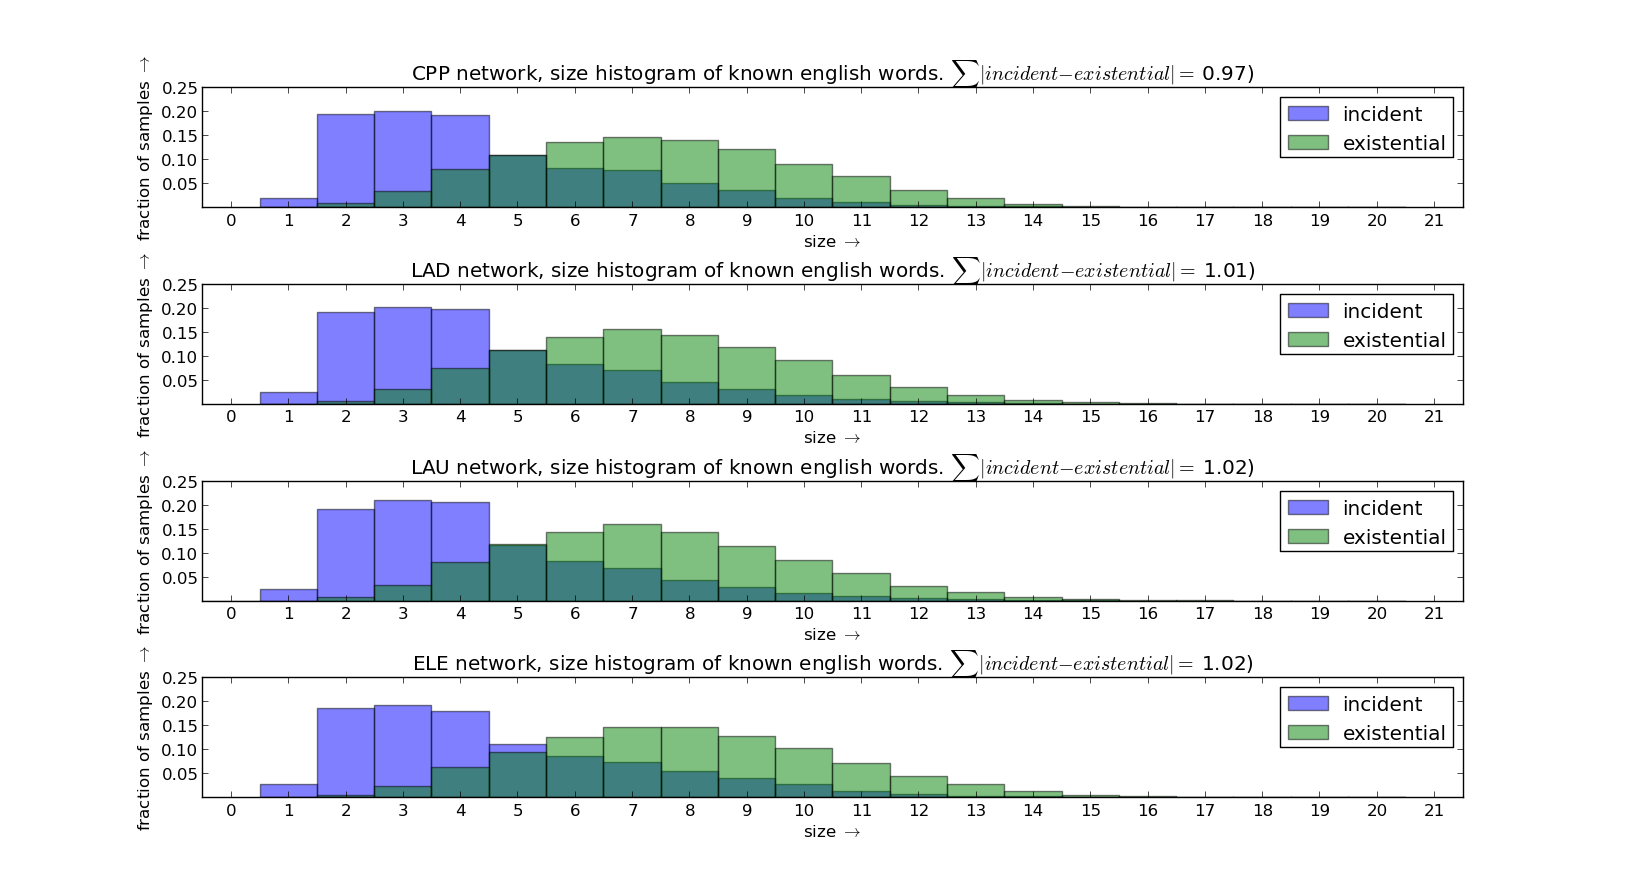
\includegraphics[width=\textwidth]{figs/kw}
%    \caption{Size of words that are known in English. Crossing of incident and existential sizes is around 5 (Figure~\ref{fig:kwnsw} shows a shift to length 6-7 when consider only non stopwords). Words with three letters have maximum incidence, while most words have 7 letters. See subsection~\ref{subsec:sii} for discussion and directions.}
%    \label{fig:kw}
%\end{figure*}
%
%
%\begin{figure*}[h!]
%    \centering
%    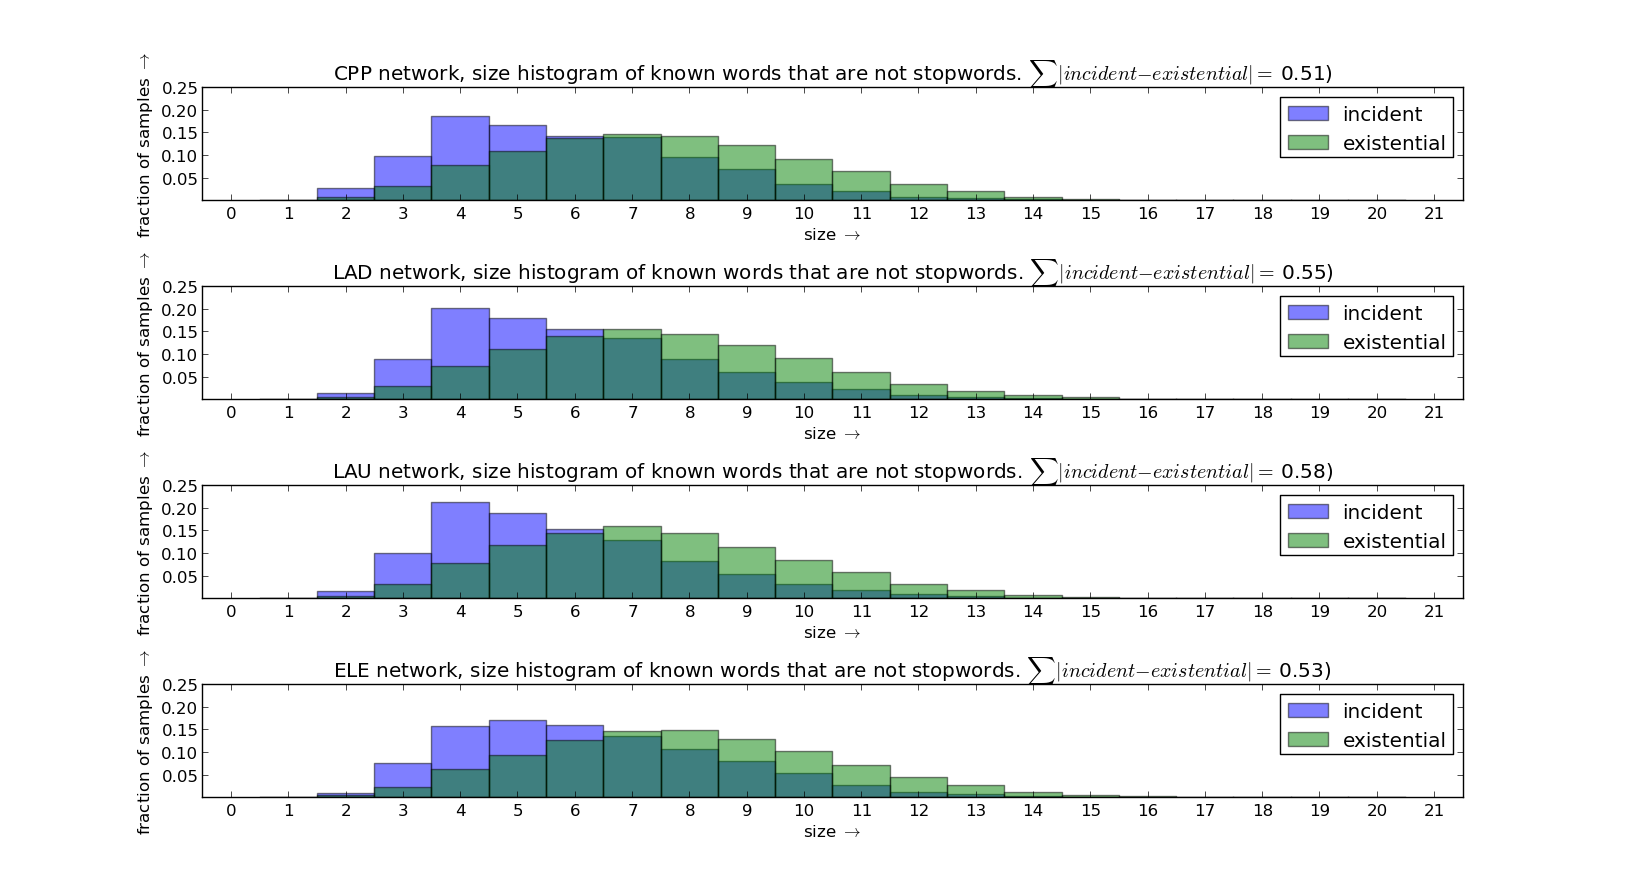
\includegraphics[width=\textwidth]{figs/kwnsw}
%    \caption{Size of words that are known in English and are not stopwords. Crossing of incident and existential sizes is around 6-7 (figure~\ref{fig:kw} shows a shift to length 5 when considered stopwords). In this case, words with 4 letters have maximum incidence, while most words still have 7 letters. Exception for ELE, which exhibits maximum incidence of words with 5 letters and most words having 8 letters, which might be associated with ELE network typology discussed in tables~\ref{tab:tokens} and~\label{tab:caracteres}. See subsection~\ref{subsec:sii} for discussion and directions.}
%    \label{fig:kwnsw}
%\end{figure*}
%
%\begin{figure*}[h!]
%    \centering
%    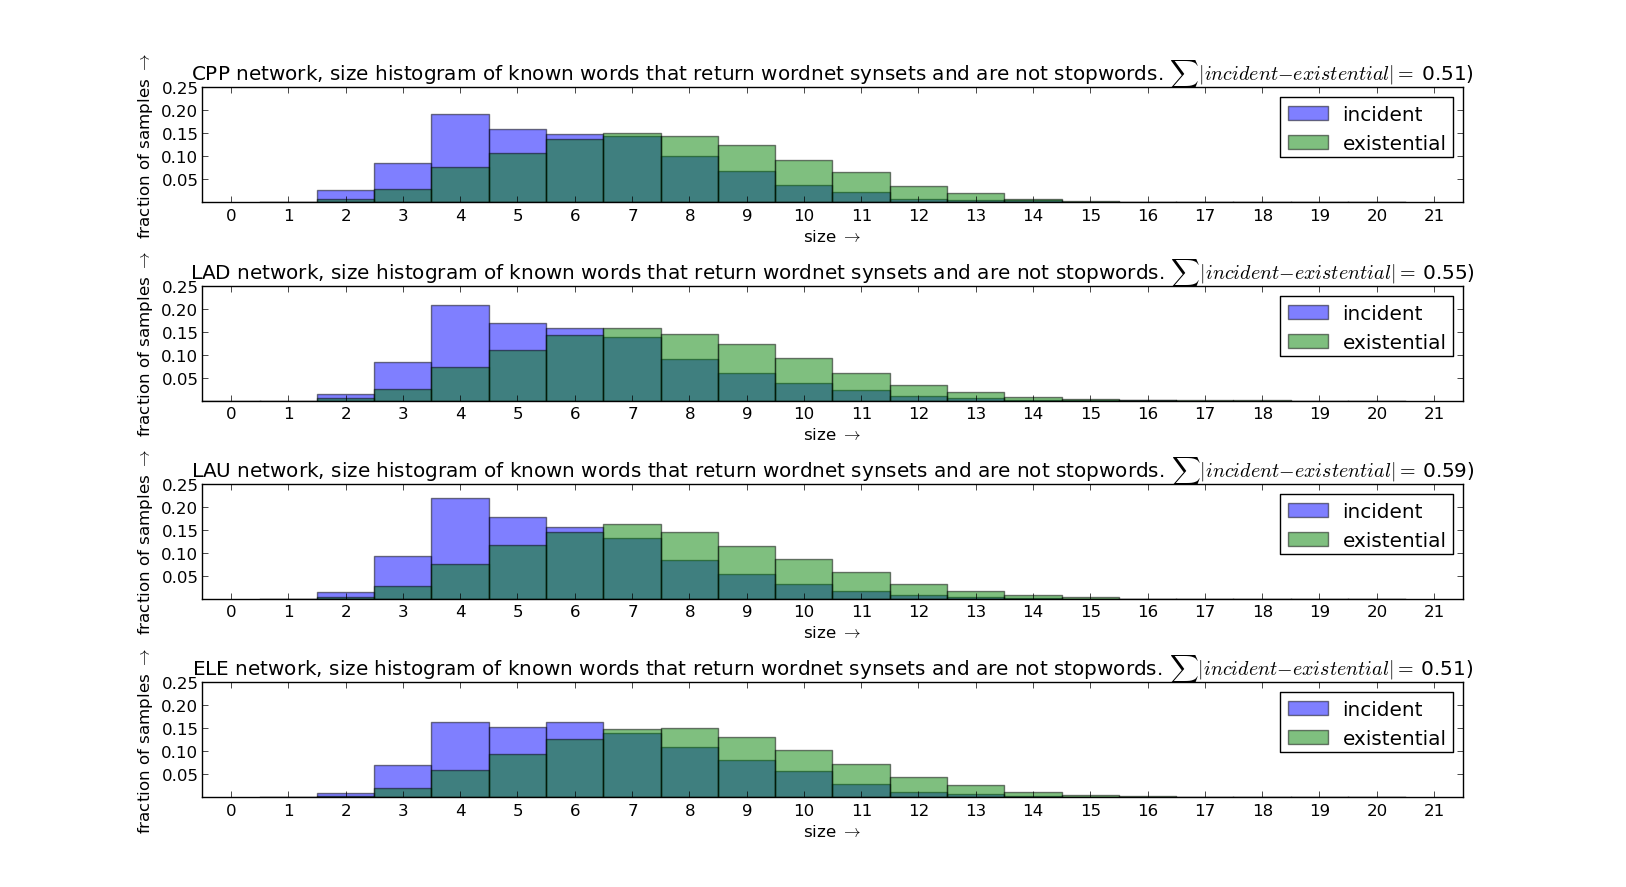
\includegraphics[width=\textwidth]{figs/kwssnsw}
%    \caption{Size of words that are known, are not stopwords and have synsets. Resembles figure~\ref{fig:kwnsw}. Stopword sizes histogram are in figure~\ref{fig:sw}. Differences suggests $\approx 0.5$ might be constant. LAD and LAU exquisite vocabulary (GNU/Linux, programming, sound/signal processing, music) might be responsible for higher difference of distributions. See subsection~\ref{subsec:sii} for discussion and directions. See subsection~\ref{subsec:sii} for discussion and directions.}
%    \label{fig:kwssnsw}
%\end{figure*}
%
%
%\begin{figure*}[h!]
%    \centering
%    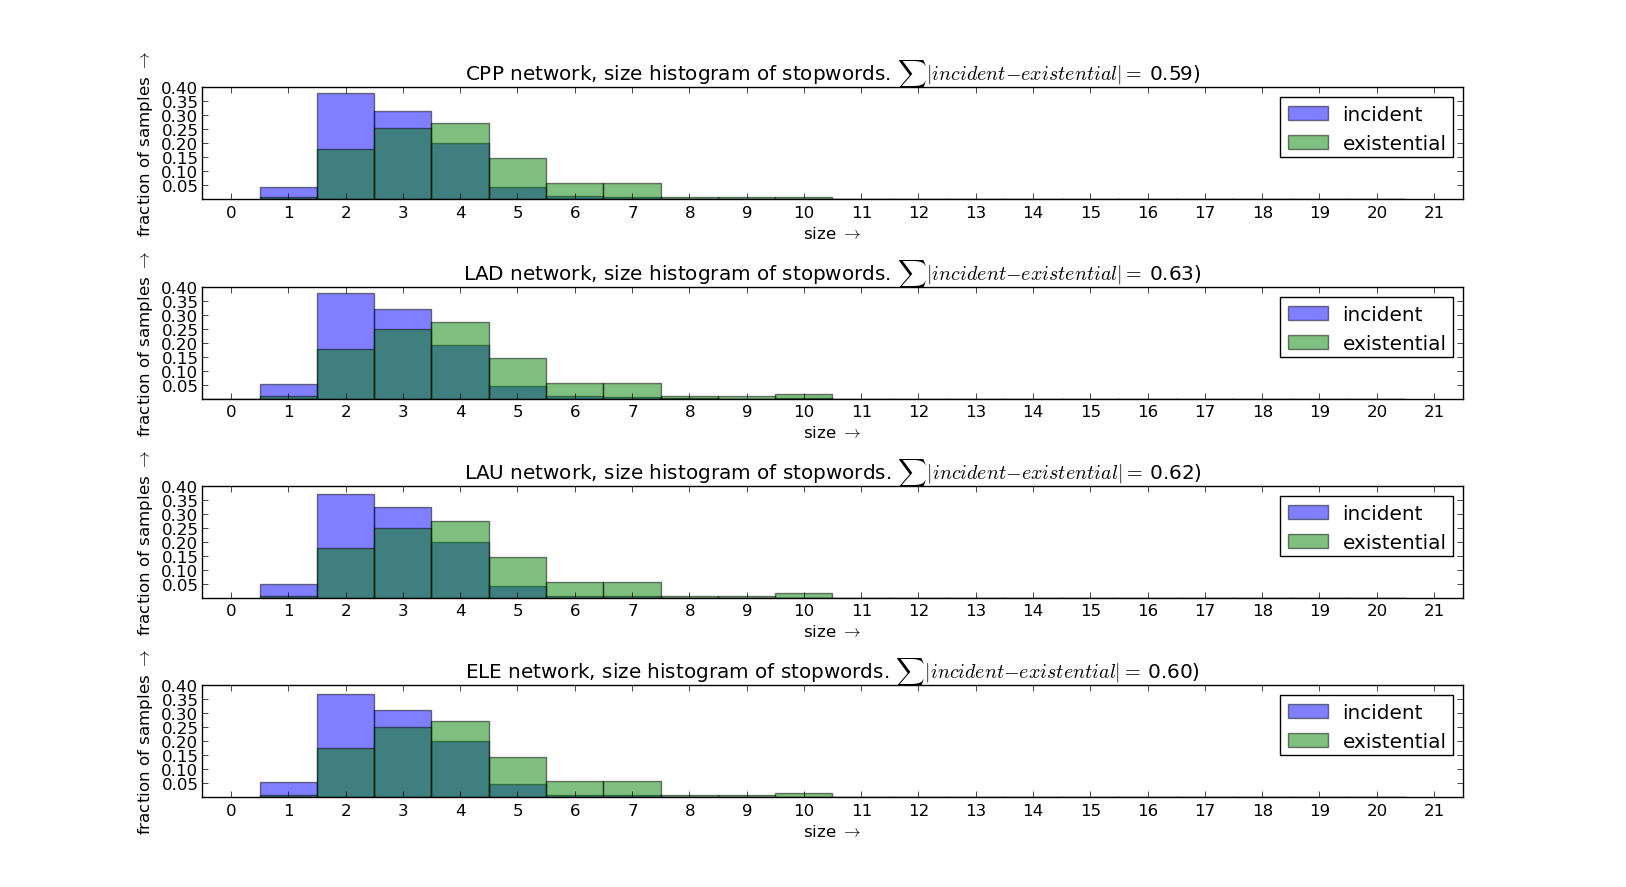
\includegraphics[width=\textwidth]{figs/sw}
%    \caption{Size histogram of stopwords. Stopwords with two letters are the most frequent, while most of them have four letters. Differences in distribution seem stable around $\approx 0.6$. See subsection~\ref{subsec:sii} for discussion and directions.}
%    \label{fig:sw}
%\end{figure*}
%
%
%
%\begin{figure*}[h!]
%    \centering
%    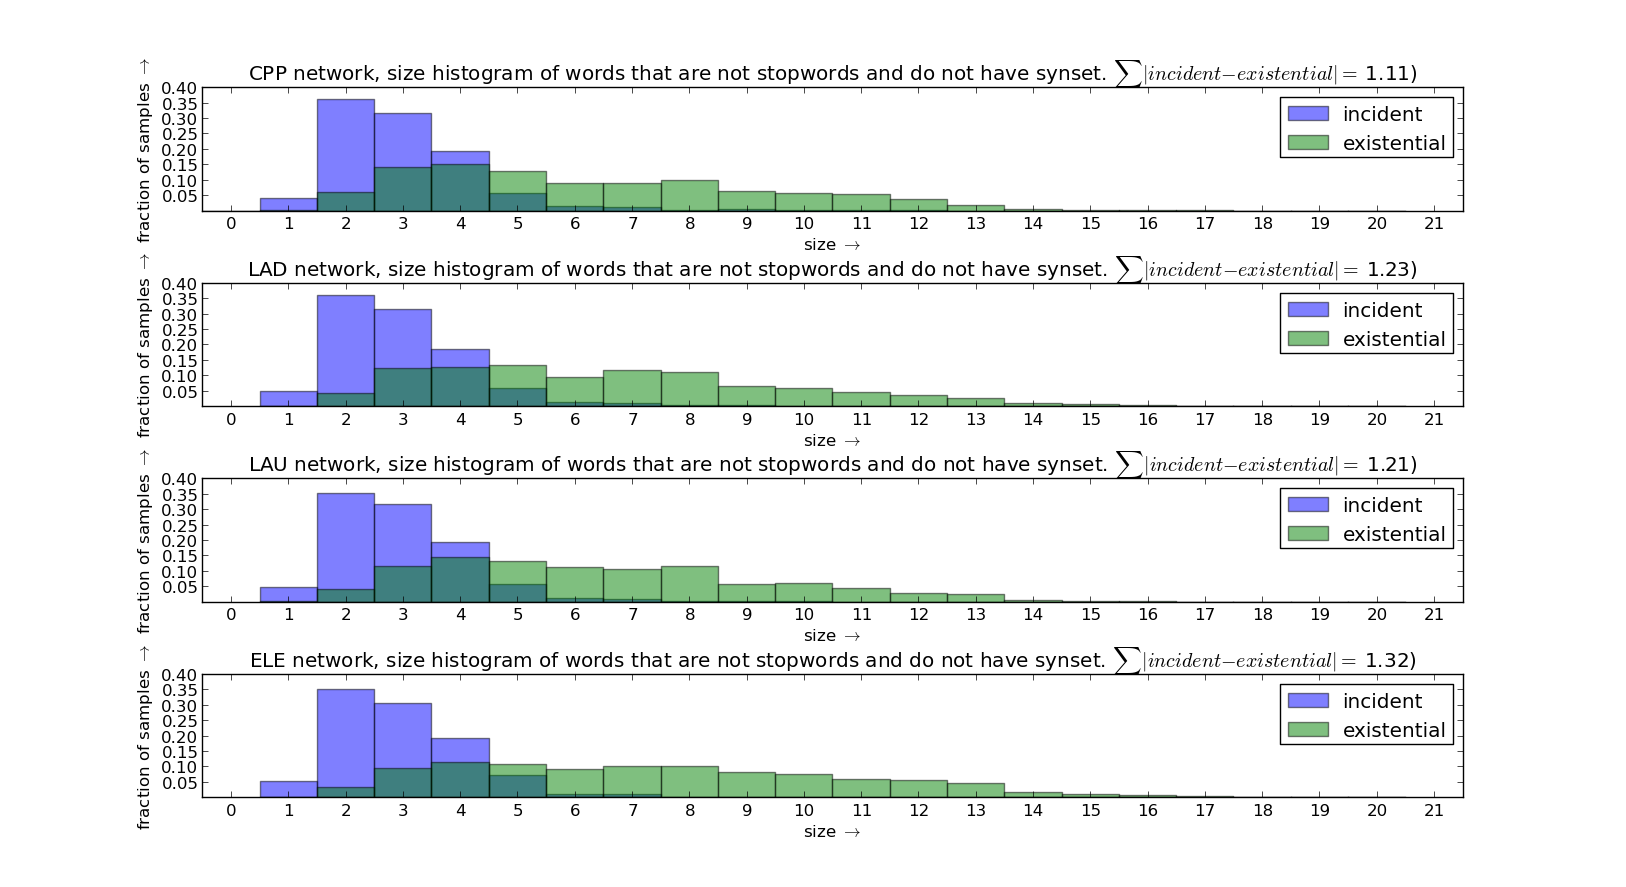
\includegraphics[width=\textwidth]{figs/nssnsw}
%    \caption{Size histogram of known English words that are not stopwords and do not return synsets. Differences in distribution suggests less stable behavior, with high incidence of few words high number of existing words with many letters. Observe difference $\geq 1$, as observed only with all known words, but even higher. See subsection~\ref{subsec:sii} for discussion and directions.}
%    \label{fig:nssnsw}
%\end{figure*}
%
%



%\newpage
%\pagebreak
\clearpage
%\nocite{*}
\bibliography{supportingInformation}% Produces the bibliography via BibTeX.
\end{document}
%
% ****** End of file aipsamp.tex ******


